\documentclass[sigconf]{acmart}

\AtBeginDocument{%
  \providecommand\BibTeX{{\normalfont B\kern-0.5em{\scshape i\kern-0.25em b}\kern-0.25em T\kern-0.1667em\lower.7ex\hbox{E}\kern-0.125emX}}
}

%% Bibliography style/data
\bibliographystyle{ACM-Reference-Format}
\citestyle{acmauthoryear}

%% Listings for inline code snippets (Python/formula excerpts from the codebase)
\usepackage{listings}
\usepackage{xcolor}
\lstdefinestyle{plem}{
  basicstyle=\ttfamily\footnotesize,
  breaklines=true,
  columns=fullflexible,
  keywordstyle=\color{blue!60!black},
  commentstyle=\color{gray},
  showstringspaces=false,
  frame=single,
  framesep=3pt,
  xleftmargin=3pt,
  xrightmargin=3pt,
}
\lstset{style=plem}

\usepackage{booktabs}
\usepackage{amsmath}
\usepackage{amssymb}
\usepackage{graphicx}

%% Copyright/rights block -- placeholder values, fill in at submission time.
\setcopyright{acmlicensed}
\copyrightyear{2026}
\acmYear{2026}
\acmDOI{10.1145/XXXXXXX.XXXXXXX}

\acmConference[SIGSPATIAL '26]{The 34th ACM SIGSPATIAL International Conference on Advances in Geographic Information Systems}{November 3--6, 2026}{Riverside, CA, USA}
\acmBooktitle{The 34th ACM SIGSPATIAL International Conference on Advances in Geographic Information Systems (SIGSPATIAL '26), November 3--6, 2026, Riverside, CA, USA}
\acmISBN{978-1-4503-XXXX-X/26/11}

\begin{document}

\title{PLEM: Polygonal Linear Evaluation Metric}
\subtitle{Evaluation Metrics and a Differentiable Training Loss for Joint Point, Linear, and Polygonal Map Feature Extraction}

\author{Daniel George}
\email{dzgeorge@usc.edu}
\affiliation{%
  \institution{University of Southern California, Viterbi School of Engineering}
  \city{Los Angeles}
  \state{CA}
  \country{USA}
}

\author{John Krumm}
\email{jkrumm@usc.edu}
\affiliation{%
  \institution{University of Southern California, Viterbi School of Engineering}
  \city{Los Angeles}
  \state{CA}
  \country{USA}
}

\begin{abstract}
Pixel intersection-over-union (IoU) is the wrong evaluation tool for linear features such as
roads: a small centerline offset or a width error collapses the score even when the extracted
road network is geometrically and topologically correct. We first introduce DTAF1, a
distance-tolerant, per-class F1 score built on tolerance-radius matching via Euclidean distance
transforms and class-agnostic across road, building, and point classes, and CBHM, a harmonic-mean
composite of centerline Dice (clDice) and boundary F1 deliberately designed as DTAF1's harsh foil.
Applying both to real SpaceNet and ISPRS Potsdam imagery surfaced two failure modes, each fixed
with an additive, non-breaking companion metric: \texttt{cbhm\_soft} (area-weighted,
non-collapsing) and DTAF1-Topo (a raster-skeleton APLS connectivity term closing DTAF1's
road-breakage blind spot). Building on this evaluation vocabulary, we then ask a training
question: can a single model learn to predict point (0D), linear (1D), and polygonal (2D) map
features \emph{jointly}, using a loss shaped by the same tolerance/topology/instance-matching
considerations that motivate these metrics, rather than a geometry-agnostic per-pixel loss? We
introduce \texttt{PLEMMultiTaskLoss}, a differentiable multi-task training loss combining three
geometry-aware terms --- a soft tolerance-band term (DTAF1 analog), a soft-clDice term (Shit
et~al.'s soft-skeletonization), and a CenterNet-style Gaussian-heatmap term standing in for
Hungarian-matched point F1, which has no tractable differentiable relaxation --- plus a masked
multi-source training scheme letting heterogeneous single-modality datasets (SpaceNet:
road+building; Potsdam: building+point) jointly supervise one 4-class model. We validate the loss
with 20 unit tests, synthetic per-term ablation sweeps confirming each term encodes the geometric
sensitivity it claims to, and a small real joint-training pipeline sanity check across 153 real
tiles, confirming all four loss terms learn jointly and that point-feature evaluation flows
end-to-end through the metric library on a real trained model's output.
\end{abstract}

\begin{CCSXML}
<ccs2012>
   <concept>
       <concept_id>10002951.10003317.10003338</concept_id>
       <concept_desc>Information systems~Geographic information systems</concept_desc>
       <concept_significance>500</concept_significance>
       </concept>
   <concept>
       <concept_id>10002951.10003317.10003347.10003350</concept_id>
       <concept_desc>Information systems~Evaluation of retrieval results</concept_desc>
       <concept_significance>500</concept_significance>
       </concept>
   <concept>
       <concept_id>10003752.10003809.10010031</concept_id>
       <concept_desc>Theory of computation~Computational geometry</concept_desc>
       <concept_significance>300</concept_significance>
       </concept>
   <concept>
       <concept_id>10010147.10010257.10010293.10010294</concept_id>
       <concept_desc>Computing methodologies~Neural networks</concept_desc>
       <concept_significance>500</concept_significance>
       </concept>
   <concept>
       <concept_id>10010147.10010257.10010293.10010294</concept_id>
       <concept_desc>Computing methodologies~Image segmentation</concept_desc>
       <concept_significance>500</concept_significance>
       </concept>
 </ccs2012>
\end{CCSXML}

\ccsdesc[500]{Information systems~Geographic information systems}
\ccsdesc[500]{Information systems~Evaluation of retrieval results}
\ccsdesc[300]{Theory of computation~Computational geometry}
\ccsdesc[500]{Computing methodologies~Neural networks}
\ccsdesc[500]{Computing methodologies~Image segmentation}

\keywords{geospatial segmentation evaluation, road extraction, building extraction,
tolerance-radius metrics, topology-aware metrics, centerline Dice, boundary F1, Average Path
Length Similarity, multiclass segmentation, differentiable loss functions, multi-task learning,
point/keypoint detection, soft-skeletonization}


\maketitle

\section{Introduction}
\label{sec:intro}

Segmentation maps of overhead imagery routinely mix feature types with fundamentally different
geometry: \emph{linear} features such as roads, one-dimensional structures extruded to a small
width; \emph{polygonal} features such as building footprints, genuinely two-dimensional regions;
and optionally \emph{point} features --- trees, lamp posts, manhole covers --- small discrete
objects spanning only a handful of pixels. A single evaluation tile covering a city block can
legitimately contain all three. Yet the standard tool for scoring segmentation quality, pixel IoU,
treats every class identically as a region-overlap problem, and that assumption breaks down
specifically for the linear case: because a road is only a few pixels wide, IoU denominators are
dominated by exactly the pixels most sensitive to sub-pixel-scale registration noise, centerline
jitter, and predicted-width error, none of which reflect whether the road network was actually
extracted correctly. The same problem recurs one level up: the \emph{training} losses
conventionally used for multiclass segmentation (cross-entropy, soft Dice) are exactly as
geometry-agnostic as IoU is as an evaluation tool --- they have no notion of tolerance, centerline
topology, or point-instance identity either, so a model trained with them has no direct pressure to
get those properties right, only to match pixels.

Table~\ref{tab:failure-modes} previews five concrete scenarios on a controlled $128\times128$
synthetic scene (a 3px-wide vertical road stripe plus a $40\times40$ building rectangle; full
setup in Section~\ref{sec:motivation}), with values computed directly against the live metrics
library for this paper. It shows where IoU's verdict diverges from actual prediction quality, and
--- importantly --- a case where \textbf{DTAF1 itself is fooled} even though it was designed to
fix IoU's problem: at 33\% random road-pixel deletion, DTAF1 still reports a perfect
$\mathbf{1.000}$, motivating DTAF1-Topo in Section~\ref{sec:topological}.

\begin{table*}
  \caption{IoU and DTAF1 failure modes for linear and polygonal features.}
  \label{tab:failure-modes}
  \begin{tabular}{@{}lccccc l@{}}
    \toprule
    Scenario & Road IoU & clDice & DTAF1 & CBHM & CBHM-soft & Correct read \\
    \midrule
    Perfect prediction & 1.000 & 1.000 & 1.000 & 1.000 & 1.000 & baseline \\
    Road shifted 5px & 0.000 & 0.000 & \textbf{1.000} & 0.000 & 0.806 &
      centerline correct; IoU/CBHM wrongly fail it \\
    Road $3.3\times$ too thick (10px vs.\ 3px GT) & 0.281 & 1.000 & 1.000 & 1.000 & 1.000 &
      centerline correct, only width wrong \\
    Road 33\% pixels deleted & 0.667 & 0.759 & \textbf{1.000} & 0.863 & 0.953 &
      network degraded; \textbf{DTAF1 misses this} \\
    Building eroded 5px & $0.562^\dagger$ & --- & 0.917 & 0.939 & 0.907 &
      shape genuinely worse; both degrade correctly \\
    Sparse road (15px offset, ${\sim}0.4\%$ of image) & 0.000 & --- & 0.500 & \textbf{0.000} & 1.000 &
      building perfect, road wrong; CBHM collapse \\
    Null prediction & 0.000 & 0.000 & 0.000 & 0.000 & 0.000 & baseline \\
    \bottomrule
  \end{tabular}
  \vspace{2pt}
  {\footnotesize $^\dagger$Building IoU, not road IoU, for this row.}
\end{table*}

We adopt a simple, uniform data representation throughout: every input is an $H\times W$
\texttt{uint8} NumPy array of integer class labels, with $0=$ background, $1=$ road, $2=$
building, and an optional $3=$ point feature, used only where the underlying dataset actually has
a point class. Every distance-based tolerance in the library is expressed in pixels but is meant
to be tied to a tile's ground sample distance (GSD): $d = \text{physical\_metres} /
\text{GSD\_metres\_per\_pixel}$, so the same physical tolerance (e.g., ``3 metres of road
centerline slop'') applies consistently across imagery captured at different resolutions.
Section~\ref{sec:method} reuses this exact class convention on batched torch tensors --- channel
index equals class id --- so a \texttt{class\_config} dict is literally shareable between an eval
call (\texttt{dtaf1()}) and a training loss (\texttt{ToleranceBandLoss}).

This paper makes seven contributions:

\begin{enumerate}
  \item \textbf{A differentiable multi-task training loss} (Section~\ref{sec:method}) whose three
    geometric terms are direct, well-precedented relaxations of three of this paper's own eval
    metrics --- soft tolerance-band (DTAF1), soft-clDice (Shit et~al.\ \cite{shit2021cldice}), and
    Gaussian-heatmap point regression (CenterNet-style) --- plus a masked multi-source training
    scheme letting heterogeneous datasets (SpaceNet road+building, Potsdam building+point) jointly
    supervise one 4-class model despite neither alone annotating all three feature types.
    Validated via controlled synthetic ablations (Section~\ref{sec:results}) and a small real
    joint-training sanity check across 153 real tiles (Section~\ref{sec:results}) --- not a
    benchmark-scale study.
  \item \textbf{DTAF1} (Section~\ref{sec:evalprotocol}) --- a single, class-agnostic
    tolerance-radius F1 formula spanning linear and polygonal classes with one code path; scoring
    a newly added feature type is a configuration change, not a code change.
  \item \textbf{CBHM} (Section~\ref{sec:evalprotocol}) --- a harmonic-mean composite of clDice and
    boundary F1, deliberately designed as DTAF1's ``harsh'' foil, so a single feature type failing
    outright is not masked by the other type succeeding.
  \item \textbf{\texttt{dtaf1\_weighted} / \texttt{cbhm\_soft}} (Section~\ref{sec:composite}) ---
    GT-pixel-count-weighted companions to DTAF1 and CBHM that soften single-class collapse,
    motivated by a real failure case found on SpaceNet imagery (\texttt{Khartoum\_img371}).
  \item A raster-only approximation of \textbf{APLS} (Section~\ref{sec:evalprotocol}) --- no
    vector road graph survives anywhere in this pipeline, see Section~\ref{sec:implementation} ---
    and \textbf{DTAF1-Topo} (Section~\ref{sec:topological}), which blends this connectivity term
    into DTAF1 and closes the road-breakage blind spot demonstrated in
    Table~\ref{tab:failure-modes}.
  \item \textbf{\texttt{point\_f1}} (Section~\ref{sec:evalprotocol}), a point-feature metric using
    Hungarian instance matching rather than greedy nearest-neighbor assignment, avoiding a
    specific adversarial failure mode.
  \item Empirical validation (Sections~\ref{sec:expsetup}--\ref{sec:results}) spanning nine
    synthetic eval-metric sensitivity sweeps, seven synthetic loss-ablation sweeps, a curated
    real-data sample from SpaceNet (four cities) and ISPRS Potsdam, and a first trained-model
    pipeline scored end-to-end by the library.
\end{enumerate}

The rest of the paper is organized as follows. Section~\ref{sec:related} places this work relative
to prior evaluation metrics and differentiable segmentation losses. Section~\ref{sec:evalprotocol}
defines each eval metric primitive, following a one-subsection-per-primitive structure.
Section~\ref{sec:motivation} empirically motivates why these primitives are necessary.
Sections~\ref{sec:composite} and~\ref{sec:topological} present two analysis-and-design studies ---
composite robustness and topological robustness. Section~\ref{sec:method} introduces the
differentiable multi-task training loss, presenting each term as a direct analog of one primitive
from Section~\ref{sec:evalprotocol}. Section~\ref{sec:implementation} describes the
implementation. Sections~\ref{sec:expsetup}--\ref{sec:results} give the full experimental setup
and results across synthetic eval sweeps, synthetic loss ablations, real-data, and trained-model
settings. Section~\ref{sec:discussion} discusses limitations honestly. Section~\ref{sec:conclusion}
concludes.

\section{Related Work}
\label{sec:related}

\subsection{IoU-family segmentation metrics}
The region-overlap baseline this paper argues against for linear features. Region-overlap IoU is
the incumbent evaluation convention across general-purpose semantic-segmentation benchmarks ---
PASCAL VOC \cite{everingham2010pascalvoc} and Cityscapes \cite{cordts2016cityscapes} --- neither of
which contains a thin, 1-pixel-wide linear class, so neither benchmark's own leaderboard practice
had to confront IoU's road-width sensitivity at all. \textbf{Motivational baseline (see also
Section~\ref{subsec:related-roads}):} on the ISPRS Potsdam benchmark
\cite{rottensteiner2012isprs,rottensteiner2014isprs}, which \emph{does} include a building class
close in kind to PLEM's polygon classes, modern models report mean IoU up to ${\sim}86\%$ and mean
F1 up to ${\sim}92\%$ --- i.e.\ plain region-overlap metrics are already near-saturated on
well-behaved polygon classes. This is the same ``good-looking score, hidden failure mode'' pattern
Section~\ref{subsec:related-roads}'s road numbers show more starkly, and is why this paper does not
treat a high IoU/F1 figure alone as evidence a metric is adequate for PLEM's target feature types.

\subsection{Topology-/skeleton-aware metrics for linear structures}
clDice and related centerline methods (Shit et~al., CVPR 2021 \cite{shit2021cldice}).

\subsection{Boundary-based metrics for polygonal features}
Boundary F1 / BF score (Csurka et~al., BMVC 2013 \cite{csurka2013evaluation}).

\subsection{Road-network extraction and connectivity metrics}
\label{subsec:related-roads}
APLS (the SpaceNet road-extraction challenge metric \cite{vanetten2018spacenet}) and TOPO
(Biagioni \& Eriksson \cite{biagioni2012topo}), the two dominant graph-connectivity metrics for
linear road networks, motivate Sections~\ref{subsec:apls} and~\ref{sec:topological}'s
\texttt{apls}/\texttt{dtaf1\_topo} primitives. \textbf{Motivational baseline:} published
road-extraction leaderboards plateau well short of 1.0 even at their best --- SpaceNet Challenge
3's winning submission scored APLS 0.666 (field topped out ${\approx}0.67$); CRESI, the
best-known raster-to-graph pipeline, reaches APLS $0.69 \pm 0.02$ \cite{vanetten2019cresi};
D-LinkNet, winner of the DeepGlobe 2018 Road Extraction Challenge, reports pixel-IoU 0.647 (val) /
0.634 (test) \cite{zhou2018dlinknet} --- a \emph{pixel}-only ceiling that says nothing about
whether the extracted network stays connected. SpaceNet's building-footprint challenges show the
same pattern from the other direction: the first SpaceNet building challenge topped out at F1
0.26, and the four-city SpaceNet~2 challenge's winner reached F1 0.693 averaged across cities
(both per \cite{vanetten2018spacenet} and the associated challenge results reporting). These are
cited here as \textbf{motivating context, not as numbers PLEM's own trained models are benchmarked
against} --- PLEM's joint-training notebooks evaluate a small curated tile subset under this
paper's own protocol, not the official SpaceNet/DeepGlobe/Potsdam test sets, so the two sets of
numbers are not directly comparable. The point of citing them is narrower and stronger than a
leaderboard comparison: even the \emph{best} published pixel/topology scores on real road and
building extraction plateau in the 0.26--0.93 range depending on class and difficulty, and a
single scalar in that range cannot by itself distinguish scattered pixel noise within tolerance
from a genuinely fragmented network --- exactly the gap \texttt{dtaf1\_topo}/\texttt{apls} close
(see the road-breakage finding in Section~\ref{sec:topological}, where \texttt{dtaf1} stays pinned
at 1.0 under 75\% real road-pixel deletion while \texttt{dtaf1\_topo}/\texttt{apls} collapse
sharply).

\subsection{Point/instance detection metrics}
COCO-style average precision \cite{lin2014coco}, and the optimal bipartite-matching literature
underlying \texttt{point\_f1}'s Hungarian assignment. Citation target: Kuhn, 1955 (the Hungarian
algorithm) \cite{kuhn1955hungarian}.

\subsection{Composite/multi-task segmentation evaluation}
Positions the gap PLEM's \emph{evaluation} half fills: existing work evaluates linear and
polygonal feature types with separate, non-comparable metrics rather than a single class-agnostic
formula (DTAF1) plus a deliberately harsh cross-type composite (CBHM).

\subsection{Differentiable segmentation losses}
\label{subsec:related-losses}
The training-side analog of the gap the previous subsection describes on the eval side. Standard
multiclass segmentation losses (cross-entropy, soft Dice --- citation target: Milletari et~al.,
3DV 2016, ``V-Net'' \cite{milletari2016vnet}) are geometry-agnostic in exactly the sense
Section~\ref{sec:intro} argues IoU is: no notion of positional tolerance, centerline topology, or
point-instance identity. Three prior lines of work each address one of those properties in
isolation, none jointly:
\begin{enumerate}
  \item \textbf{Boundary-/Hausdorff-distance losses}, which precompute a GT-side distance
    transform and use it as a fixed per-pixel weight against the model's soft output --- citation
    targets: Kervadec et~al., 2019 (``Boundary loss for highly unbalanced segmentation'')
    \cite{kervadec2019boundary}; Karimi \& Salcudean, 2019 (Hausdorff-distance loss)
    \cite{karimi2019hausdorff} --- the direct precedent for Section~\ref{subsec:tolerance-loss}'s
    soft tolerance-band term.
  \item \textbf{Soft-clDice}, a differentiable soft-skeletonization loss for tubular structures ---
    citation target: Shit et~al., CVPR 2021 \cite{shit2021cldice} (the same paper cited for clDice
    itself in Section~\ref{subsec:cldice} --- here cited for its \emph{loss}, not its eval metric,
    contribution) --- the direct precedent for Section~\ref{subsec:cldice-loss}.
  \item \textbf{Heatmap regression for keypoint/point detection}, which reformulates discrete
    point detection as dense Gaussian-target regression rather than an instance-matching problem
    --- citation targets: Law \& Deng, ECCV 2018 (``CornerNet'') \cite{law2018cornernet};
    Zhou et~al., 2019 (``CenterNet''/``Objects as Points'') \cite{zhou2019centernet} --- the
    direct precedent for Section~\ref{subsec:heatmap-loss}.
\end{enumerate}
Section~\ref{sec:method}'s contribution is combining well-precedented individual relaxations of
(1)--(3) into one multi-task loss covering all three geometric properties simultaneously, plus the
masked multi-source training scheme (Section~\ref{subsec:multitask-loss}) that lets two datasets
which individually annotate only two of the three feature types jointly supervise one model.

\section{Evaluation Protocol}
\label{sec:evalprotocol}

These six primitives now serve two purposes rather than one: as before, they are PLEM's
evaluation vocabulary for scoring any prediction against ground truth; as of
Section~\ref{sec:method}, three of them are also the metric each corresponds to that a
differentiable loss term is designed to approximate during training. Nothing in this section
changes to accommodate that --- the metrics stay exactly as originally defined and validated;
Section~\ref{sec:method} does the work of relating a \emph{separate} differentiable formulation
back to each one.

\textbf{Shared notation.} Let $P$ and $G$ be $H\times W$ integer label maps (prediction and
ground truth) over the class set $C = \{0, 1, 2, [3]\}$. For class $c$, define binary masks
$P_c = (P = c)$ and $G_c = (G = c)$. Every primitive in this section is applied per-class and then
reduced (macro or GT-pixel-count-weighted mean) across the classes relevant to it.

\textbf{Shared edge-case convention.} Every primitive below implements the same rule, verified
identical across \texttt{dtaf1.py:43-51}, \texttt{cldice.py:51-56}, \texttt{boundary\_f1.py:68-72},
\texttt{point\_f1.py:109-120}, and \texttt{apls.py:141-144}:
both $P_c$ and $G_c$ empty $\Rightarrow$ score $= 1.0$ (vacuously correct); exactly one of $P_c,
G_c$ empty $\Rightarrow$ score $= 0.0$ (total failure). Stated once here as a cross-cutting design
decision rather than repeated per metric.

\subsection{DTAF1 --- Distance-Tolerant, per-class F1}
\label{subsec:dtaf1}

Tolerance-radius matching via Euclidean distance transforms
(\texttt{scipy.ndimage.distance\_transform\_edt}):
\begin{align}
  \mathrm{TP}_{\mathrm{pred}} &= |\{x \in P_c : \mathrm{EDT}(1-G_c)(x) \le d_c\}| \\
  \mathrm{TP}_{\mathrm{gt}}   &= |\{x \in G_c : \mathrm{EDT}(1-P_c)(x) \le d_c\}| \\
  \mathrm{Precision}_c &= \mathrm{TP}_{\mathrm{pred}} / |P_c|, \quad
  \mathrm{Recall}_c = \mathrm{TP}_{\mathrm{gt}} / |G_c| \\
  F1_c &= \frac{2 \cdot \mathrm{Precision}_c \cdot \mathrm{Recall}_c}
               {\mathrm{Precision}_c + \mathrm{Recall}_c}
\end{align}
Reduction across classes (both are always computed; \texttt{reduction} just selects which is
surfaced as the top-level \texttt{dtaf1} key):
\begin{align}
  \mathrm{DTAF1}_{\mathrm{macro}} &= \tfrac{1}{|C|}\textstyle\sum_c F1_c \\
  \mathrm{DTAF1}_{\mathrm{weighted}} &= \left(\textstyle\sum_c n_c F1_c\right) \big/
    \left(\textstyle\sum_c n_c\right), \quad n_c = |G_c|
\end{align}

\begin{lstlisting}[language=Python, caption={Tolerance-matching core, \texttt{metrics/dtaf1.py:53-64}}]
dist_from_gt = distance_transform_edt(1 - g)
dist_from_pred = distance_transform_edt(1 - p)
tp_pred = int(((p == 1) & (dist_from_gt <= d)).sum())
tp_gt = int(((g == 1) & (dist_from_pred <= d)).sum())
precision = tp_pred / n_pred
recall = tp_gt / n_gt
f1 = (2 * precision * recall / (precision + recall)
      if (precision + recall) > 0 else 0.0)
\end{lstlisting}

\texttt{DEFAULT\_TOLERANCES = \{"road": 10, "building": 2\}} (pixels; see
Section~\ref{subsec:tolerance-radii} for how these were chosen). Function signature:
\texttt{dtaf1(pred, gt, class\_config, reduction="macro") -> dict}, returning \texttt{dtaf1},
\texttt{dtaf1\_macro}, \texttt{dtaf1\_weighted}, \texttt{per\_class}. \textbf{Class-agnostic by
construction} --- scoring a new class costs zero code changes, just an added
\texttt{class\_config} entry. Section~\ref{subsec:tolerance-loss}'s \texttt{ToleranceBandLoss}
reuses this exact \texttt{class\_config} shape.

\subsection{clDice --- Centerline Dice}
\label{subsec:cldice}

(Cite Shit et~al., CVPR 2021 \cite{shit2021cldice} in Section~\ref{sec:related} --- not here.)
\begin{align}
  S_p &= \mathrm{skeletonize}(P_c), \quad S_g = \mathrm{skeletonize}(G_c) \\
  T_{\mathrm{prec}} &= |S_p \cap G_c| / |S_p|, \quad T_{\mathrm{sens}} = |S_g \cap P_c| / |S_g| \\
  \mathrm{clDice} &= \frac{2 \cdot T_{\mathrm{prec}} \cdot T_{\mathrm{sens}}}
                          {T_{\mathrm{prec}} + T_{\mathrm{sens}}}
\end{align}
Width-insensitive (a predicted road $3.3\times$ too thick still scores $\mathrm{clDice}=1.000$,
Table~\ref{tab:failure-modes} row 2) but offset-brittle: skeletons of the exact same road shifted
5px share \emph{zero} overlap ($\mathrm{clDice}=0.000$, row 1) --- this offset-sensitivity is
exactly what motivates DTAF1's distance-tolerant matching instead of a raw skeleton intersection.
Section~\ref{subsec:cldice-loss}'s \texttt{SoftClDiceLoss} reimplements this width-insensitivity
property differentiably, with a caveat (Sections~\ref{subsec:cldice-loss},~\ref{sec:discussion}).

\subsection{Boundary F1 (BF) and the IoU Baseline}
\label{subsec:bf}

(Cite Csurka et~al., BMVC 2013 \cite{csurka2013evaluation} in Section~\ref{sec:related} --- not
here.)
\begin{align}
  \mathrm{Precision} &= |\{x \in B_p : \mathrm{dist}(x, B_g) \le \tau\}| / |B_p| \\
  \mathrm{Recall} &= |\{x \in B_g : \mathrm{dist}(x, B_p) \le \tau\}| / |B_g| \\
  \mathrm{BF} &= \frac{2 \cdot \mathrm{Precision} \cdot \mathrm{Recall}}
                      {\mathrm{Precision} + \mathrm{Recall}}
\end{align}
where $B_p = \mathrm{boundary}(P_c)$, $B_g = \mathrm{boundary}(G_c)$ via morphological boundary
extraction. \texttt{iou()} is introduced here explicitly as the pixel-overlap baseline comparator
used throughout Sections~\ref{sec:motivation} and~\ref{sec:expsetup}. Section~\ref{subsec:boundary-loss}'s
\texttt{SoftBoundaryLoss} reuses Section~\ref{subsec:tolerance-loss}'s precision/recall primitive
applied to a soft boundary map instead of the full class mask, making it the most directly-shared
piece of machinery between any two \texttt{losses/} terms.

\subsection{Point F1 --- Hungarian Instance Matching}
\label{subsec:pointf1}

For the optional point class (trees, lamp posts, manhole covers): connected-component blobs are
reduced to centroids (\texttt{scipy.ndimage.label} + \texttt{center\_of\_mass}), then matched via
tolerance-restricted Hungarian assignment (\texttt{scipy.optimize.linear\_sum\_assignment}), not
greedy nearest-neighbor.

\begin{lstlisting}[language=Python, caption={Hungarian assignment core, \texttt{metrics/point\_f1.py:58-65}}]
dist = cdist(gt_c, pred_c)
big = tolerance * 1e6 + 1.0
cost = np.where(dist <= tolerance, dist, big)
row_ind, col_ind = linear_sum_assignment(cost)
valid = dist[row_ind, col_ind] <= tolerance
return int(valid.sum())
\end{lstlisting}

Justified by the clustered-points adversarial case in \texttt{TestPointInstanceMatching}: greedy
nearest-neighbor gets $\mathrm{TP}=1$ where Hungarian finds the globally optimal $\mathrm{TP}=2$
(formalized in Appendix~\ref{app:proofs}, Section~\ref{app:a6}). \textbf{This is the one primitive
with no differentiable analog in Section~\ref{sec:method}} --- Hungarian assignment and
connected-component labeling have no useful gradient path back to per-pixel logits;
Section~\ref{subsec:heatmap-loss} reformulates point supervision entirely as heatmap regression
instead, a genuine train/eval formulation mismatch discussed explicitly in
Section~\ref{sec:discussion}.

\subsection{APLS --- Raster-Skeleton Average Path Length Similarity}
\label{subsec:apls}

No vector road graph survives anywhere in this pipeline --- \texttt{datasets/common.py::rasterize\_lines}
collapses roads straight to a flat pixel mask, discarding segment/graph structure --- so APLS is
approximated entirely from raster skeletons (\texttt{metrics/apls.py}): skeletonize pred/GT masks,
build an 8-connected pixel-adjacency graph (\texttt{networkx}; edge weight = Euclidean pixel
distance), then for sampled GT control-point pairs $(u,v)$ within one GT connected component,
compare GT shortest-path length $L_{\mathrm{gt}}(u,v)$ against the predicted shortest-path length
between the nearest snap-matched predicted-graph nodes (\texttt{scipy.spatial.cKDTree}), scoring
$\max(0, 1 - |L_{\mathrm{pred}} - L_{\mathrm{gt}}| / L_{\mathrm{gt}})$ if matched, else 0.
Control-point pairs are sampled \textbf{grouped by source}, so one
\texttt{nx.single\_source\_dijkstra\_path\_length} call amortizes across many targets instead of
one independent Dijkstra call per pair --- see complexity analysis in
Appendix~\ref{app:complexity}, Section~\ref{app:b6}. This is deliberately sensitive to a failure
DTAF1's per-pixel tolerance matching misses entirely: once the skeleton fragments, shortest paths
between control points either lengthen sharply or vanish, so APLS collapses where DTAF1 does not.
\textbf{Graph shortest-path recomputation has no tractable lightweight differentiable relaxation}
(Section~\ref{sec:method}'s design assessment, Section~\ref{sec:discussion}) --- APLS and
DTAF1-Topo (Section~\ref{sec:topological}) stay eval-only permanently, a stated design decision
rather than a to-do.

\subsection{CBHM --- Composite clDice/Boundary-F1 Harmonic Mean}
\label{subsec:cbhm}

\begin{align}
  \mathrm{clDice}_{\mathrm{mean}} &= \mathrm{mean}(\mathrm{clDice}_c : c \in \mathrm{linear\_classes}) \\
  \mathrm{BF}_{\mathrm{mean}} &= \mathrm{mean}(\mathrm{BF}_c : c \in \mathrm{polygon\_classes}) \\
  \mathrm{CBHM} &= \frac{2 \cdot \mathrm{clDice}_{\mathrm{mean}} \cdot \mathrm{BF}_{\mathrm{mean}}}
                        {\mathrm{clDice}_{\mathrm{mean}} + \mathrm{BF}_{\mathrm{mean}}}
\end{align}
The harmonic mean is a \textbf{deliberate design choice}: a single class scoring 0 collapses the
whole composite to 0. Positioned explicitly as the ``harsh'' foil to DTAF1's more lenient macro
average (Table~\ref{tab:failure-modes}'s ``Road shifted 5px'' row: $\mathrm{DTAF1}=1.000$ but
$\mathrm{CBHM}=0.000$, on the \emph{same} input).

\textbf{Composition note.} These six primitives compose into the two ``final iteration''
composites covered later rather than here --- \texttt{cbhm\_soft} in Section~\ref{sec:composite}
and DTAF1-Topo in Section~\ref{sec:topological} --- and, as of this revision, into the three
geometry-aware \texttt{losses/} terms in Section~\ref{sec:method}.

\section{Why These Metrics? Empirical Motivation}
\label{sec:motivation}

A controlled experiment showing the baseline tool fails, followed by an interpretation of why.

\subsection{Experimental Setup}
\label{subsec:motivation-setup}

All numbers in this section come from the $128\times128$ synthetic scene defined in
\texttt{notebooks/metric\_comparison.ipynb}: a 3px-wide vertical road stripe (class 1) through the
tile center, plus a $40\times40$ building rectangle (class 2) in the upper-left quadrant. Nine
sweep functions in \texttt{tests/test\_sensitivity.py} perturb this scene along one axis at a
time (Table~\ref{tab:sweeps}).

\begin{table}
  \caption{Synthetic sensitivity sweeps (\texttt{tests/test\_sensitivity.py}).}
  \label{tab:sweeps}
  \begin{tabular}{@{}lll@{}}
    \toprule
    Sweep & Perturbs & Range \\
    \midrule
    \texttt{sweep\_road\_offset} & horizontal road shift & 0--24px \\
    \texttt{sweep\_road\_breakage} & random road pixel dropout & 0--100\% \\
    \texttt{sweep\_building\_erosion} & building erosion radius & 0--11px \\
    \texttt{sweep\_road\_thickness} & predicted road thickness & 1--21px \\
    \texttt{sweep\_class\_imbalance} & road:building GT ratio & 0.4--3.1\% \\
    \texttt{sweep\_sparse\_class\_offset} & sparse road offset & 0--20px \\
    \texttt{sweep\_point\_jitter} & horizontal point shift & 0--20px \\
    \texttt{sweep\_point\_dropout} & fraction points removed & 0--100\% \\
    \texttt{sweep\_point\_clutter} & spurious points added & 0--20 \\
    \bottomrule
  \end{tabular}
\end{table}

Section~\ref{subsec:lossablation-setup} introduces a tenth family,
\texttt{tests/test\_loss\_sensitivity.py}, that reuses these exact same scenes/perturbation
functions (imported directly, not duplicated) to sweep the \emph{loss} side instead.

\subsection{Results}
\label{subsec:motivation-results}

Table~\ref{tab:failure-modes} is reproduced from a direct run of the library against this scene.
Three additional single-axis sweeps sharpen the picture:

\textbf{Road offset sweep} (tolerance $=10$px): Road IoU and clDice both collapse to $0.000$
immediately at offset $=4$px, while DTAF1 stays at $1.000$ through offset $=10$px exactly at its
tolerance boundary, then degrades --- $0.667$ at 12px, $0.500$ from 16px onward (the building's
still-perfect class dragging the macro average).

\textbf{Road breakage sweep} (seed 42): Road IoU degrades roughly linearly with dropout fraction
($1.000 \to 0.500$ at 50\% $\to 0.201$ at 80\%), clDice degrades faster and less evenly, but
\textbf{DTAF1 remains pinned at exactly $1.000$ for every dropout fraction from 0\% through 90\%},
only dropping (to $0.500$) once 100\% of road pixels are gone. This is the blind spot in its
starkest form: DTAF1 cannot distinguish a perfectly intact road from one with 90\% of its pixels
randomly deleted, because the surviving pixels are scattered widely enough that some surviving
pixel still falls within the 10px tolerance radius of nearly every GT pixel.

\textbf{Road thickness sweep} (GT fixed at 3px): Road IoU falls from $1.000$ at correct thickness
to $0.157$ at 21px predicted thickness, while both clDice and DTAF1 stay at $1.000$ through 13px
and only start softening at very extreme over-thickness --- confirming width-insensitivity holds
over a wide practical range.

\textbf{Building erosion sweep}: all three metrics degrade together and roughly proportionally
with erosion radius (Building IoU $1.000{\to}0.203$, BF $1.000{\to}0.512$, DTAF1
$1.000{\to}0.728$ at radius 11) --- the one scenario where IoU's verdict was never wrong to begin
with, included as a control.

\subsection{Interpretation via Distance-Transform Geometry}
\label{subsec:motivation-interpretation}

DTAF1's tolerance radius $d_c$ defines, for every pixel, a disc of admissible positional error: a
predicted pixel counts as correct if \emph{any} GT pixel of the same class lies within $d_c$, and
vice versa for recall. This is precisely why width and small-offset errors are absorbed: every
pixel of an over-thick or slightly-shifted road still has some true road pixel within $d_c$, so
precision and recall both stay near 1. The same geometry is also precisely why DTAF1 is blind to
breakage: the tolerance radius has no notion of \emph{which} surviving pixels are connected to
each other --- it only asks ``is there a same-class pixel nearby,'' a purely local, per-pixel
question. Random dropout removes pixels roughly uniformly, so even at high dropout fractions the
\emph{remaining} pixels tend to still lie within $d_c$ of most GT locations, exactly as a spatial
Poisson-thinning argument would predict: for a road of width $w$ and tolerance $d_c \gg w$, the
probability that some surviving pixel lies within $d_c$ of a given GT pixel stays high until the
surviving fraction becomes small relative to $w/d_c$. clDice does encode a \emph{global}
connectivity signal (via skeletonization), which is why it degrades faster and less evenly than
DTAF1 under the same dropout sweep --- but clDice's zero-tolerance to any positional offset makes
it unusable as DTAF1's replacement outright. This tension --- a tolerance radius that must be wide
enough to absorb positional/width noise but is then necessarily blind to the connectivity question
at that same radius --- is the structural reason a \emph{separate} connectivity term (APLS,
Section~\ref{subsec:apls}) is needed rather than simply shrinking $d_c$; Section~\ref{sec:topological}
develops this formally, and Section~\ref{sec:method} shows the same ``wide enough to absorb noise,
blind to connectivity'' tradeoff reproduces itself on the training-loss side
(\texttt{ToleranceBandLoss} has no connectivity term either, by the same design logic).

\section{Analysis and Design for Composite Robustness}
\label{sec:composite}

A controlled-complexity task family, an efficient corrective proxy, then a parameter-design
application.

\subsection{Class-Imbalance--Controlled Tasks}
\label{subsec:class-imbalance}

\texttt{sweep\_class\_imbalance} and \texttt{sweep\_sparse\_class\_offset} parameterize a
controlled-complexity axis: instead of varying a task's spatial frequency, we vary the road's
\emph{share of GT pixels} (0.4--3.1\% in \texttt{sweep\_class\_imbalance}, with the road entirely
missing from the prediction) or its \emph{offset} (\texttt{sweep\_sparse\_class\_offset}, road
share fixed at ${\sim}0.4\%$). In both sweeps, \texttt{cbhm} (harsh, harmonic) sits at exactly
$0.000$ for every non-trivial perturbation level, while \texttt{cbhm\_soft} tracks the dominant
(building) class instead, staying between $0.758$ and $1.000$ across the same ranges. As a scalar
summary, define the \textbf{harsh-composite collapse threshold}: the smallest perturbation
magnitude at which \texttt{cbhm} first reaches exactly 0. Empirically this threshold is
effectively immediate --- \texttt{cbhm}'s harmonic mean has essentially zero tolerance once one
class is fully wrong, regardless of how small that class's share of the scene is.

\subsection{Weighted Reduction as an Efficient Corrective Proxy}
\label{subsec:weighted-reduction}

\begin{align}
  \mathrm{cbhm\_soft} = w_{\mathrm{linear}} \cdot \mathrm{clDice}_{\mathrm{mean,weighted}} +
                         w_{\mathrm{polygon}} \cdot \mathrm{BF}_{\mathrm{mean,weighted}}
\end{align}
where $w_{\mathrm{linear}} = N_{\mathrm{linear}} / (N_{\mathrm{linear}} + N_{\mathrm{polygon}})$
is each type's share of total GT pixels (0.5/0.5 if both totals are 0).

\begin{lstlisting}[language=Python, caption={\texttt{metrics/unified.py:88-102}}]
cl_mean_weighted = (float(np.dot(cldice_weights, cldice_scores) / cl_total)
                     if cl_total > 0 else 0.0)
bf_mean_weighted = (float(np.dot(bf_weights, bf_scores) / bf_total)
                     if bf_total > 0 else 0.0)
type_total = cl_total + bf_total
w_cl = float(cl_total / type_total) if type_total > 0 else 0.5
w_bf = float(bf_total / type_total) if type_total > 0 else 0.5
cbhm_soft = w_cl * cl_mean_weighted + w_bf * bf_mean_weighted
\end{lstlisting}

The key structural move: \texttt{cbhm\_soft} is a \textbf{reweighting of already-computed
per-class scores}, not a redesign of the harmonic-mean composite itself. It costs nothing beyond
the per-class scores DTAF1/CBHM already compute. \textbf{Stated carefully, not oversold}:
\texttt{cbhm\_soft} is a weighted \emph{arithmetic} mean, not geometric --- a geometric mean still
collapses to exactly 0 whenever one input is 0, same as harmonic (formalized in
Appendix~\ref{app:proofs}, Sections~\ref{app:a3}--\ref{app:a4}).

\textbf{Worked example --- the real failure that motivated this fix.} On real SpaceNet imagery
(\texttt{composite\_vs\_submetric\_report.ipynb}, tile \texttt{Khartoum\_img371}), a 12px road
offset gave $\mathrm{cbhm}=0.000$ despite $\mathrm{dtaf1}=0.934$ (per-class road F1 $=0.867$,
precision $=0.872$, recall $=0.863$) --- the road is only ${\sim}0.1\%$ of image pixels, and
clDice collapsed entirely on this sparse, offset road, dragging the harmonic mean to exactly zero
even though the dominant building class was essentially perfect. \texttt{cbhm\_soft} recovers
only partially here ($0.000 \to \mathbf{0.285}$), because the road actually has \emph{more} GT
pixels than the building despite its tiny share of image \emph{area} --- area-weighting only
helps when the failing class is also the pixel-count minority. Contrast
\texttt{Khartoum\_img333}, where the building genuinely dominates by pixel count: $\mathrm{cbhm}$
$0.48$--$0.52 \to \mathrm{cbhm\_soft}$ $\mathbf{0.85}$, a clean recovery. This nuance is treated as
a real limitation, not a clean win --- expanded in Section~\ref{sec:discussion}.

\subsection{Choosing Per-Class Tolerance Radii}
\label{subsec:tolerance-radii}

\texttt{DEFAULT\_TOLERANCES = \{"road": 10, "building": 2\}} (pixels) were validated, not guessed,
against the offset and erosion sweeps in Section~\ref{subsec:motivation-results}: the road offset
sweep shows DTAF1 holding at $1.000$ through exactly the 10px boundary and softening immediately
past it, confirming the tolerance behaves as intended rather than being either so tight it rejects
correct predictions or so loose it never penalizes anything. This is a cheap, already-available
sweep used as the design proxy instead of an expensive full retrain (or, here, a full real-data
re-annotation) for every candidate tolerance value --- though PLEM's tolerances are fixed
physically-motivated constants ($d = \text{physical\_metres} / \text{GSD\_metres\_per\_pixel}$)
rather than a learned/optimized parameter; Section~\ref{sec:conclusion} lists learned/adaptive
tolerance radii as future work. Section~\ref{subsec:tolerance-loss}'s \texttt{ToleranceBandLoss}
reuses these same tolerance values directly via a shared \texttt{class\_config}.

\section{Analysis and Design for Topological Robustness}
\label{sec:topological}

A structural property the primitive lacks, a sensitivity analysis, then a closed-form-plus-numerical
design section.

\subsection{The Connectivity Blind Spot}
\label{subsec:blindspot}

This subsection formally states a property DTAF1 \textbf{lacks}: pointwise EDT tolerance-matching
is not ``connectivity-injective.'' Concretely (proof sketch; full statement in
Appendix~\ref{app:proofs}):

\begin{quote}
For a road mask $G_c$ of width $w$ and tolerance $d_c$, there exist predicted masks $P_c$ obtained
from $G_c$ by deleting an arbitrarily large fraction of pixels --- up to and including masks in
which $G_c$'s connected skeleton is fully disconnected into many isolated fragments --- such that
$\mathrm{DTAF1}_c(P_c, G_c) = 1.0$, provided the surviving pixels remain within $d_c$ of every GT
pixel.
\end{quote}

Section~\ref{subsec:motivation-results}'s road-breakage sweep is the empirical witness: DTAF1
stays at exactly $1.000$ through 90\% random dropout on the synthetic scene.

\subsection{APLS as Connectivity Recovery, and Its Sensitivity to Fragmentation}
\label{subsec:apls-recovery}

APLS (Section~\ref{subsec:apls}) recovers exactly the signal DTAF1 lacks: its score depends on
shortest-path length \emph{between} control points, not merely on point-to-point proximity, so it
is sensitive to whether a path exists at all. Framing the dropout fraction as the ``noise'' axis,
the empirical curve has a two-regime character: a near-flat, low-sensitivity regime while the
skeleton is still mostly connected, followed by a sharp departure once fragmentation actually
occurs (Table~\ref{tab:breakage-topo}).

\begin{table}
  \caption{Road-breakage sweep: DTAF1 vs.\ CBHM vs.\ APLS vs.\ DTAF1-Topo.}
  \label{tab:breakage-topo}
  \begin{tabular}{@{}lcccc@{}}
    \toprule
    Dropout & \texttt{dtaf1} & \texttt{cbhm} & \texttt{road\_apls} & \texttt{dtaf1\_topo} \\
    \midrule
    0.0 & 1.000 & 1.000 & 1.000 & 1.000 \\
    0.1 & 1.000 & 0.965 & 0.898 & 0.946 \\
    0.2 & 1.000 & 0.919 & 0.883 & 0.938 \\
    0.3 & 1.000 & 0.909 & \textbf{0.247} & \textbf{0.397} \\
    0.5 & 1.000 & 0.805 & 0.029 & 0.057 \\
    0.7 & 1.000 & 0.606 & 0.005 & 0.010 \\
    1.0 & 0.500 & 0.000 & 0.000 & 0.000 \\
    \bottomrule
  \end{tabular}
\end{table}

The transition is sharp between 0.2 and 0.3: \texttt{road\_apls} falls from $0.883$ to $0.247$ in
that one step --- the point at which the road skeleton's largest connected fragment actually
detaches from enough control-point pairs that shortest paths start disappearing rather than merely
lengthening. \texttt{dtaf1} shows no analogous transition anywhere in the swept range.

\subsection{Harmonic-Blending Design for DTAF1-Topo}
\label{subsec:dtaf1topo}

\begin{lstlisting}[language=Python, caption={Blending primitive, \texttt{metrics/dtaf1\_topo.py:29-31,74-87}}]
def _harmonic_mean(a, b):
    denom = a + b
    return float(2 * a * b / denom) if denom > 0 else 0.0

# per class in linear_classes:
entry["blended"] = _harmonic_mean(base["f1"], a)  # a = apls
# non-linear classes keep entry["blended"] = base["f1"]
\end{lstlisting}

\subsubsection{Closed-Form Boundary Behavior}

The harmonic mean of $F1$ and $\mathrm{APLS}$ has a simple, exactly-analyzable shape at its
boundaries:
\begin{itemize}
  \item $\mathrm{APLS}=0, F1=1$ (the DTAF1 blind-spot regime, worst case): $\mathrm{blended}=0$. A
    perfectly tolerance-matched but fully disconnected road scores exactly zero once blended,
    regardless of how high $F1$ is.
  \item $\mathrm{APLS}=1, F1=1$: $\mathrm{blended}=1$, recovering DTAF1's own perfect score
    unchanged.
  \item For fixed $F1=1$, $\mathrm{blended}(\mathrm{APLS}) = 2\mathrm{APLS}/(1+\mathrm{APLS})$ ---
    concave and always $\le \mathrm{APLS}$, meaning the harmonic blend never \emph{rewards}
    connectivity beyond what APLS itself reports; it can only ever penalize a
    topologically-correct-looking $F1$ down toward the (generally lower) APLS score, never the
    reverse. This asymmetry is intentional: it is the mechanism by which DTAF1-Topo closes the
    blind spot rather than merely averaging two independent opinions.
\end{itemize}

\subsubsection{Numerical Validation via the Road-Breakage Sweep}

Unlike the closed-form boundary analysis above, the \emph{practical} question --- where along the
dropout axis does the blend actually diverge from plain DTAF1? --- has no closed form and is
answered numerically. Table~\ref{tab:breakage-topo} already gives the answer directly:
\texttt{dtaf1\_topo} tracks \texttt{road\_apls} closely (both driven to near-zero by fraction
0.5--0.7) while \texttt{dtaf1} stays at $1.000$ throughout --- this \emph{is} the fix, cross-checked
against the assertions in \texttt{tests/test\_metrics\_sanity.py::TestRoadBreakageRegression}.
\textbf{Validated on synthetic data only} --- see Section~\ref{sec:discussion} for the real-data
caveat.

\medskip
\noindent\textbf{Bridge to Section~\ref{sec:method}.} Every property analyzed so far --- offset
tolerance (Section~\ref{subsec:dtaf1}), width insensitivity (Section~\ref{subsec:cldice}),
connectivity/breakage sensitivity (this section), instance-level point matching
(Section~\ref{subsec:pointf1}) --- was developed purely as an \emph{evaluation} concern: a
property a \emph{finished} prediction is scored against, after training is already done.
Section~\ref{sec:method} asks the natural next question: if these are the geometric properties
that actually distinguish a good extraction from a bad one, why train a model with a loss that has
no notion of any of them? The three tractable properties (tolerance, width-insensitivity via
topology, point-instance-like localization) are exactly the three \texttt{losses/} implements as
differentiable training terms; the one property with no tractable differentiable relaxation (graph
connectivity, this section) is exactly the one \texttt{losses/} leaves out, by design, not
oversight.

\section{A Differentiable Multi-Task Loss for Joint 0D/1D/2D Extraction}
\label{sec:method}

Sections~\ref{sec:evalprotocol}--\ref{sec:topological} are eval-only by construction: DTAF1,
Boundary F1, and APLS are built on \texttt{scipy.ndimage.distance\_transform\_edt}; clDice on
\texttt{skimage.morphology.skeletonize}; Point F1 on
\texttt{scipy.optimize.linear\_sum\_assignment}. Every one of these operations is discrete and
breaks autograd, so none of them can be used directly as a training loss. This section introduces
\texttt{losses/}, a new top-level package (parallel to \texttt{metrics/} and \texttt{datasets/},
pure \texttt{torch}) of differentiable training losses, each a direct analog of one primitive from
Section~\ref{sec:evalprotocol} --- mirrored in spirit, never sharing code with its eval-side
counterpart (numpy+scipy vs.\ torch tensors inside an autograd graph cannot share an
implementation) --- so a single model can be trained to \emph{jointly} predict point (0D), linear
(1D), and polygonal (2D) map features using a loss shaped by the same tolerance, topology, and
instance-matching considerations Sections~\ref{sec:evalprotocol}--\ref{sec:topological} spent five
sections motivating.

\subsection{Design Principle: Differentiable Analogs, Not Shared Code}
\label{subsec:method-principle}

\texttt{losses/} operates on the standard PyTorch segmentation convention --- $(B,C,H,W)$ logits,
$(B,H,W)$ int64 label maps, channel index equal to class id --- not Section~\ref{sec:evalprotocol}'s
$H\times W$ numpy label-map convention. Table~\ref{tab:correspondence} summarizes the
correspondence and, for each term, what had to change relative to its eval-metric counterpart to
make it differentiable.

\begin{table*}
  \caption{Eval metric $\leftrightarrow$ differentiable loss term correspondence.}
  \label{tab:correspondence}
  \begin{tabular}{@{}p{2.7cm}p{2.7cm}p{10.5cm}@{}}
    \toprule
    Eval metric & \texttt{losses/} term & What changed to make it differentiable \\
    \midrule
    DTAF1 (\S\ref{subsec:dtaf1}) & \texttt{ToleranceBandLoss} (\S\ref{subsec:tolerance-loss}) &
      GT-side dilation-by-radius precomputed once per batch (GT is a fixed target, not a model
      output); the harder \emph{recall} direction --- which needs an EDT of the \emph{prediction}
      on the eval side --- is made differentiable by soft-dilating the model's own continuous
      probability map via iterated max-pool instead of a detached hard threshold. \textbf{Both}
      precision and recall stay fully differentiable; no stop-gradient approximation was needed on
      either term, a stronger result than initially assessed necessary (\S\ref{sec:discussion}). \\
    Boundary F1 (\S\ref{subsec:bf}) & \texttt{SoftBoundaryLoss} (\S\ref{subsec:boundary-loss}) &
      Soft boundary map $=$ morphological gradient $\mathrm{dilate}(x) - \mathrm{erode}(x)$
      (saturates to exactly 1.0 at a hard edge --- an early $|x-\mathrm{avgpool}(x)|$ formulation
      was tried and rejected, since its peak response is well below 1.0 and silently caps
      achievable recall even under perfect alignment); reuses \texttt{ToleranceBandLoss}'s
      precision/recall primitive on this soft boundary map instead of the full class mask. \\
    clDice (\S\ref{subsec:cldice}) & \texttt{SoftClDiceLoss} (\S\ref{subsec:cldice-loss}) &
      Shit et~al.'s (2021) soft-skeletonization: iterated soft-erode/soft-open via
      max-pool/min-pool, applied directly to the probability map --- no discrete
      \texttt{skeletonize} call. Runs for a \emph{fixed} iteration count rather than to
      convergence, so width-invariance is bounded (\S\ref{subsec:cldice-loss},
      \S\ref{sec:discussion}), unlike the eval-side metric. \\
    Point F1 (\S\ref{subsec:pointf1}) & \texttt{PointHeatmapLoss} (\S\ref{subsec:heatmap-loss}) &
      \textbf{Not a relaxation.} Hungarian assignment and connected-component labeling have no
      useful gradient path. Reformulated entirely as CenterNet-style dense Gaussian-heatmap
      regression --- a genuinely different formulation, not a softened version of the eval
      metric's algorithm. \\
    APLS / DTAF1-Topo (\S\ref{subsec:apls}/\S\ref{subsec:dtaf1topo}) & \emph{(none)} & No
      tractable lightweight differentiable relaxation of graph shortest-path recomputation
      exists; stays eval-only permanently --- a stated design decision
      (\S\ref{sec:discussion}), not a gap to be filled later. \\
    \bottomrule
  \end{tabular}
\end{table*}

\texttt{PLEMMultiTaskLoss} (Section~\ref{subsec:multitask-loss}) combines the first three, with
\texttt{class\_config} reused verbatim from \texttt{dtaf1.py}'s convention
(Section~\ref{subsec:dtaf1}) --- the same dict can be passed to \texttt{dtaf1()} for evaluation
and \texttt{ToleranceBandLoss} for training.

\subsection{Soft Tolerance-Band Loss (DTAF1 Analog)}
\label{subsec:tolerance-loss}

Recall that DTAF1's precision test only requires a distance transform \emph{from GT}, while its
recall test requires one \emph{from the prediction}. This asymmetry turns out to matter: precision
needs only a GT-side dilation-by-$d$ mask (equivalent to $\mathrm{dist\_from\_gt} \le d$), which is
fixed target construction and can be precomputed once per batch under \texttt{no\_grad}. Recall is
the harder direction on the eval side because it distance-transforms the \emph{prediction} ---
but since \texttt{F.max\_pool2d} is differentiable, applying it directly and iteratively to the
model's own soft probability map (``soft-dilating'' it) keeps gradients flowing with no detach:
\begin{align}
  \mathrm{gt\_band}_c &= \mathrm{dilate}(G_c, d_c) \quad \text{(precomputed, no\_grad)} \\
  \mathrm{precision}_c &= \frac{\sum(p_c \cdot \mathrm{gt\_band}_c) + \epsilon}{\sum(p_c) + \epsilon} \\
  \mathrm{recall}_c &= \frac{\sum(g_c \cdot \mathrm{soft\_dilate}(p_c, d_c)) + \epsilon}{\sum(g_c) + \epsilon} \\
  \mathrm{loss}_c &= w(1-\mathrm{precision}_c) + (1-w)(1-\mathrm{recall}_c)
\end{align}
where $p_c$ is the model's softmax probability for class $c$ and $g_c$ is the one-hot GT mask.
Both denominators use epsilon smoothing (matching \texttt{train\_unet.ipynb}'s existing soft-Dice
convention) rather than explicit both-empty branching, so a class absent from both prediction and
GT reduces cleanly toward the ``both empty $\to$ perfect'' convention without a separate code
path.

\begin{lstlisting}[language=Python, caption={\texttt{losses/tolerance.py}}]
def soft_tolerance_pair_loss(pred_soft, gt_hard, radius, eps=1e-6, precision_weight=0.5):
    gt_band = _dilate_binary(gt_hard.unsqueeze(1), radius)[:, 0]
    dilated_pred = soft_dilate_prob(pred_soft.unsqueeze(1), radius)[:, 0]
    p_sum, g_sum = pred_soft.sum(dim=(1, 2)), gt_hard.sum(dim=(1, 2))
    prec_num = (pred_soft * gt_band).sum(dim=(1, 2))
    rec_num = (gt_hard * dilated_pred).sum(dim=(1, 2))
    precision = (prec_num + eps) / (p_sum + eps)
    recall = (rec_num + eps) / (g_sum + eps)
    loss = precision_weight * (1.0 - precision) + (1.0 - precision_weight) * (1.0 - recall)
    return loss.mean()
\end{lstlisting}

\texttt{ToleranceBandLoss} applies this per class over a \texttt{class\_config} dict of the same
\texttt{\{class\_id: \{"name", "tolerance"\}\}} shape as \texttt{dtaf1.py}'s
\texttt{ROAD\_BUILDING\_CONFIG}, macro-averaging across the configured linear + polygon classes.

\subsection{Soft Boundary Loss (Boundary F1 Analog)}
\label{subsec:boundary-loss}

The soft boundary map reuses the same soft-erode/soft-dilate primitives
Section~\ref{subsec:cldice-loss} introduces for soft-skeletonization:
$\mathrm{boundary}(x) = \mathrm{dilate}(x) - \mathrm{erode}(x)$, the morphological gradient, which
is $0$ in flat interior/exterior regions and saturates to exactly $1.0$ at a hard, confident class
edge. \texttt{SoftBoundaryLoss} then calls Section~\ref{subsec:tolerance-loss}'s
\texttt{soft\_tolerance\_pair\_loss} on this soft boundary map (predicted side) against a
thresholded boundary map of the one-hot GT (computed under \texttt{no\_grad}) instead of on the
full class mask --- the most directly-shared piece of machinery between any two \texttt{losses/}
terms, and the most mechanical of the three.

\subsection{Soft-clDice Loss (clDice Analog)}
\label{subsec:cldice-loss}

Implements Shit et~al.'s (CVPR 2021) soft-skeletonization directly: iterated
$\mathrm{soft\_erode}(x) = -\mathrm{maxpool}(-x)$ / $\mathrm{soft\_dilate}(x) = \mathrm{maxpool}(x)$
/ $\mathrm{soft\_open}(x) = \mathrm{soft\_dilate}(\mathrm{soft\_erode}(x))$, accumulating skeleton
response across scales exactly as the original paper's reference algorithm does, applied to the
model's continuous probability map instead of a discretely-\texttt{skeletonize()}d binary mask:
\begin{align}
  \mathrm{tprec}_c &= \frac{\sum(\mathrm{skel}(p_c) \cdot g_c) + \epsilon}{\sum(\mathrm{skel}(p_c)) + \epsilon} \\
  \mathrm{tsens}_c &= \frac{\sum(\mathrm{skel}(g_c) \cdot p_c) + \epsilon}{\sum(\mathrm{skel}(g_c)) + \epsilon} \\
  \mathrm{soft\_clDice}_c &= \frac{2 \cdot \mathrm{tprec}_c \cdot \mathrm{tsens}_c}
                                  {\mathrm{tprec}_c + \mathrm{tsens}_c + \epsilon}, \quad
  \mathrm{loss}_c = 1 - \mathrm{soft\_clDice}_c
\end{align}

\textbf{Known limitation, unlike the eval-side metric:} soft-skeletonization runs for a
\emph{fixed} number of iterations ($\mathrm{iters}=10$ default), not to convergence, so
width-invariance only holds up to whatever width that iteration count can fully erode away --- a
documented, iteration-bounded version of Section~\ref{subsec:cldice}'s exact width-invariance.
Validated directly: on a $32\times32$ synthetic scene, a GT road of thickness 3px scores
soft-clDice loss $4.77\times10^{-7}$ against a matching thickness-3px prediction, and \textbf{the
identical $4.77\times10^{-7}$} against a $3\times$-thicker (9px) prediction on the same centerline
--- i.e., zero measurable width sensitivity up to a $3\times$ ratio --- while plain soft Dice on
the same 9px input scores only $0.500$, confirming soft-clDice is doing something meaningfully
different from plain Dice, not just numerically saturating
(\texttt{tests/test\_losses\_sanity.py::TestSoftClDiceLoss::test\_width\_insensitivity}).

\subsection{Point-Heatmap Regression Loss (Point F1 Analog, Reformulated)}
\label{subsec:heatmap-loss}

Per Table~\ref{tab:correspondence}, this term is \textbf{not} a relaxation of
Section~\ref{subsec:pointf1}'s Hungarian matching --- connected-component labeling and
combinatorial assignment have no useful gradient. Instead, point supervision is reformulated
entirely as dense Gaussian-heatmap regression, CenterNet-style: each GT point instance's centroid
(extracted via the exact same \texttt{scipy.ndimage.label} + \texttt{center\_of\_mass} pipeline
\texttt{point\_f1.py}'s \texttt{\_instance\_centroids} already uses at eval time --- here purely
for \emph{target} construction, under \texttt{no\_grad}) is burned into a Gaussian blob on a
target heatmap (overlapping Gaussians combined via elementwise max, avoiding peak inflation where
GT points cluster), and the point class's own softmax probability channel is trained directly
against it with a penalty-reduced pixelwise focal loss (CornerNet/CenterNet formulation):
\begin{align}
  \mathrm{gt\_heatmap}(x) &= \max_{c \in \mathrm{centroids}} \exp\left(-\frac{\|x-c\|^2}{2\sigma^2}\right) \\
  \mathrm{pos\_loss}(x) &= -(1-p(x))^\alpha \log p(x) \quad \text{if } \mathrm{gt\_heatmap}(x) = 1 \\
  \mathrm{neg\_loss}(x) &= -(1-\mathrm{gt\_heatmap}(x))^\beta p(x)^\alpha \log(1-p(x)) \quad
    \text{otherwise} \\
  \mathrm{loss} &= \frac{\sum_x \mathrm{pos\_loss}(x) + \sum_x \mathrm{neg\_loss}(x)}
                        {\max(1, \mathrm{num\_positive\_pixels})}
\end{align}
\texttt{point\_f1.py}'s Hungarian matching is untouched and remains a pure eval-time metric ---
this is a genuine, documented train/eval formulation mismatch (Section~\ref{sec:discussion}), not
papered over as a relaxation.

\subsection{\texttt{PLEMMultiTaskLoss}: Combination and Multi-Source Class Masking}
\label{subsec:multitask-loss}

The combined loss sums a CE+soft-Dice base term (adapted from \texttt{train\_unet.ipynb}'s
existing \texttt{combined\_loss}) with the three geometry-aware terms above, each independently
weighted:
\begin{align}
  L = w_{\mathrm{ce\_dice}} L_{\mathrm{ce\_dice}} + w_{\mathrm{tol}} L_{\mathrm{tolerance}} +
      w_{\mathrm{cldice}} L_{\mathrm{cldice}} + w_{\mathrm{heatmap}} L_{\mathrm{heatmap}}
\end{align}

\textbf{Multi-source class masking.} SpaceNet tiles annotate road+building only (no point class
exists at SpaceNet's GSD, Section~\ref{subsec:realdata-setup}); Potsdam tiles annotate
building+point only (no road class in Potsdam's palette). Training one 4-class model on both
jointly requires each sample to be supervised only on the classes its \emph{source} actually
annotates. This is implemented by additively biasing a sample's masked-out class channels to a
large negative logit \textbf{before} any softmax is taken:
\begin{align}
  \mathrm{logits}'[:,c] = \mathrm{logits}[:,c] + (1 - \mathrm{class\_mask}[:,c]) \cdot (-10^4)
\end{align}
Since every term above is a function of softmax probabilities, driving a masked channel's
pre-softmax logit to $-\infty$ makes its post-softmax probability --- and therefore its gradient
contribution to \emph{every} term at once --- vanish identically. This is a single mechanism
shared by all four loss terms, rather than four bespoke masking implementations, and relies on
target label maps never containing a class id a sample's source doesn't annotate (true by
construction for both \texttt{datasets/spacenet.py} and \texttt{datasets/potsdam.py}'s
rasterizers, Sections~\ref{subsec:realdata-setup},~\ref{subsec:joint-setup}).
\texttt{PLEMMultiTaskLoss.forward()} returns a dict (\texttt{"loss"} plus each active sub-term as
a detached float) --- mirroring Section~\ref{sec:evalprotocol}'s ``always return a dict of named
scalars'' convention on the training side too, so per-epoch logging code looks structurally
similar to \texttt{evaluate\_all()}'s output.

\section{Implementation}
\label{sec:implementation}

\begin{itemize}
  \item All \texttt{metrics/}/\texttt{datasets/} inputs/outputs are plain NumPy $H\times W$
    \texttt{uint8} arrays --- no framework lock-in. \texttt{losses/} (Section~\ref{sec:method}) is
    the one exception by design: it is pure \texttt{torch}, batched-tensor, differentiable, and
    deliberately kept in its own top-level package rather than inside \texttt{metrics/}, whose
    documented contract (``every public function takes $H\times W$ integer label maps and returns
    dicts of named scalars'') is non-differentiable by construction --- adding torch code there
    would silently violate that invariant.
  \item Every public \texttt{metrics/}/\texttt{datasets/} function returns a \textbf{dict of named
    scalars}, never a bare float, for logging/inspection; \texttt{PLEMMultiTaskLoss.forward()}
    follows the same convention on the training side (Section~\ref{subsec:multitask-loss}).
\end{itemize}

\begin{table}
  \caption{Tech stack, grouped by role.}
  \label{tab:techstack}
  \begin{tabular}{@{}p{2.6cm}p{5.3cm}@{}}
    \toprule
    Role & Libraries \\
    \midrule
    Core numerics & \texttt{numpy}, \texttt{scipy} (\texttt{scipy.ndimage}) \\
    Skeletonization/morphology & \texttt{scikit-image} \\
    Graph algorithms & \texttt{networkx}, \texttt{scipy.spatial.cKDTree} \\
    Optimal assignment & \texttt{scipy.optimize.linear\_sum\_assignment} (eval-only) \\
    Geospatial I/O & \texttt{rasterio}, \texttt{shapely} \\
    Data acquisition & \texttt{requests} (anonymous S3), \texttt{kaggle} \\
    Differentiable training losses & \texttt{torch}/\texttt{torch.nn.functional} (CPU-only); no
      \texttt{kornia}/\texttt{torchvision} dependency added \\
    Testing/analysis & \texttt{pytest}, \texttt{pandas}, \texttt{matplotlib}, \texttt{jupyterlab} \\
    \bottomrule
  \end{tabular}
\end{table}

Package structure/exports note: \texttt{dtaf1\_topo}, \texttt{apls}/\texttt{apls\_multiclass}/
\texttt{mean\_apls} are \textbf{not} re-exported at the \texttt{metrics/\_\_init\_\_.py} top level;
\texttt{cbhm\_soft} exists only as a dict key inside \texttt{cbhm()}'s return, not a separate
function --- deliberate, framed as ``validated on synthetic data only, not yet a drop-in
replacement in the consolidated report'' (\texttt{evaluate\_all()}, expanded in
Section~\ref{sec:discussion}). \texttt{losses/\_\_init\_\_.py} re-exports all five public classes
(\texttt{ToleranceBandLoss}, \texttt{SoftBoundaryLoss}, \texttt{SoftClDiceLoss},
\texttt{PointHeatmapLoss}, \texttt{PLEMMultiTaskLoss}) --- no equivalent ``not yet wired in''
caveat, since Section~\ref{sec:method}'s terms are new and never had a prior consolidated entry
point to be missing from.

\section{Experimental Setup}
\label{sec:expsetup}

\subsection{Synthetic Benchmark}
\label{subsec:synthetic-setup}

$128\times128$ scene: vertical road stripe (class 1) + $40\times40$ building rectangle (class 2),
from \texttt{notebooks/metric\_comparison.ipynb}. The nine sweep functions listed in
Table~\ref{tab:sweeps} (\texttt{tests/test\_sensitivity.py}).

\subsection{Real-Data Sample}
\label{subsec:realdata-setup}

SpaceNet SN2 (buildings, $650\times650$px) + SN3 (roads, $1300\times1300$px) from the public
unauthenticated S3 bucket, cities Vegas/Khartoum/Paris/Shanghai, up to ${\sim}100$ tiles curated,
the two tiling grids reconciled via coarse-then-dense nearest-neighbor spatial matching, verified
by rasterized pixel overlap (not just bbox overlap). Plus ISPRS Potsdam (6cm/px) \cite{isprs-potsdam} for the point
class (trees), 15 crops via a Kaggle mirror, thresholded by palette color + connected-component
labeled.

No trained extractor was available for most of this evaluation, so ``pred'' $=$ real GT run
through the same perturbation families as the synthetic sweeps
(\texttt{notebooks/real\_data\_evaluation.ipynb}), at fixed severities: \texttt{road\_offset}
$\in\{0,4,8,12,16\}$px, \texttt{road\_dropout}$\in\{0,25,50,75\}\%$,
\texttt{road\_thicken}$\in\{0,2,4,6\}$px, \texttt{building\_erode}$\in\{0,1,2,3\}$px,
\texttt{point\_jitter}$\in\{0,3,6,10,15\}$px, \texttt{point\_dropout}$\in\{0,25,50,75,100\}\%$,
\texttt{point\_clutter}$\in\{0,5,10,15,20\}$ extra blobs.

\subsection{Trained Model (First Real Prediction Source)}
\label{subsec:trainedmodel-setup}

Small 3-level encoder/decoder U-Net, base$=16$ channels doubling per level, single softmax head
over $\{\text{bg},\text{road},\text{building}\}$, \textbf{483,475 parameters}. 100 SpaceNet tiles
split \textbf{70/15/15 at the tile level} (avoids patch-leakage inflating held-out scores),
patchified to 256px (2520 train / 540 val patches). Loss $=$ class-weighted cross-entropy $+$ soft
Dice; class weights $[0.1, 1.313, 1.602]$ for (bg, road, building), from pixel counts
$[147742496, 9565097, 7843127]$. CPU-only, 15 epochs \cite{ronneberger2015unet}. This is the
frozen CE+Dice \textbf{baseline} referenced by Section~\ref{subsec:joint-setup}'s ablation.

\textbf{Limitation stated explicitly here}: ``${\sim}100$ curated real tiles with no pretraining is
a small dataset for segmentation; treat as a pipeline sanity check, not a benchmark result.''

\subsection{Loss Ablation Setup}
\label{subsec:lossablation-setup}

Mirrors Section~\ref{subsec:motivation-setup}'s synthetic-sweep methodology exactly:
\texttt{tests/test\_loss\_sensitivity.py} imports the same scene builders and perturbed-scene
generators directly from \texttt{tests/test\_sensitivity.py} (\texttt{SHAPE}, \texttt{make\_road},
\texttt{make\_building}, \texttt{make\_gt}, \texttt{make\_points}, \texttt{GT},
\texttt{POINT\_COORDS} --- not duplicated), so every loss-side sweep perturbs the \emph{identical}
synthetic scene as its eval-metric counterpart. Rather than accuracy, each sweep records
\textbf{loss value} for a perturbed prediction against the fixed ground truth, encoded as
``confidently peaked'' logits (softmax $\approx$ one-hot at the perturbed label, but at a
moderate confidence scale) fed through \texttt{PLEMMultiTaskLoss}, reporting five configurations
built from its own sub-term breakdown: \texttt{ce\_dice\_only}, \texttt{plus\_tolerance},
\texttt{plus\_cldice}, \texttt{plus\_heatmap}, \texttt{full}. Seven sweeps mirror seven of the
nine synthetic families (road offset/breakage/thickness, building erosion, point
jitter/dropout/clutter --- \texttt{sweep\_class\_imbalance}/\texttt{sweep\_sparse\_class\_offset}
have no loss-side analog, since they are about how eval-time composite \emph{reductions} behave,
not a property of one loss term).

\textbf{Methodology note on confidence scale.} The eval-side unit tests
(Section~\ref{sec:results}, \texttt{tests/test\_losses\_sanity.py}) use a ``fully confident'' logit
encoding (softmax $\approx 1-10^{-10}$) to test perfect-prediction behavior. The loss-ablation
sweeps deliberately use a more moderate confidence scale instead (softmax $\approx 0.999$): at
full confidence, \texttt{PointHeatmapLoss}'s focal-loss log term saturates at its numerical clamp
ceiling for \emph{every} confidently-wrong pixel, and since each predicted point blob spans
multiple pixels, a handful of false-positive point predictions can inflate a sweep's total loss by
roughly two orders of magnitude --- a test-harness artifact of total confidence no real model
output actually reaches, not a property of the loss itself. This is itself a useful, real finding
for Section~\ref{subsec:joint-setup}: the heatmap term's absolute magnitude scales differently from
the other three (a CornerNet-style focal formulation, not a bounded $[0,1]$ ratio the
tolerance/clDice terms are), motivating \texttt{PLEMMultiTaskLoss}'s per-term \texttt{weights} dict
for rebalancing during real training.

\subsection{Joint Multi-Source Training Setup}
\label{subsec:joint-setup}

Neither SpaceNet nor Potsdam alone annotates all three feature types (Section~\ref{subsec:multitask-loss}):
SpaceNet supplies road+building but no point class; Potsdam's 6-class palette includes
\texttt{building} and point-capable \texttt{tree}/\texttt{car} classes but no road/linear class at
all. A genuinely joint 0D/1D/2D training run therefore requires combining both sources under
\texttt{PLEMMultiTaskLoss}'s masked multi-source scheme. \textbf{The data-side half of this is
built and validated against real data}: \texttt{datasets/potsdam.py::label\_raster\_to\_building\_mask}
extracts the \texttt{building} palette color (a straight threshold, deliberately not routed
through the point pipeline's connected-component + area filter, which would wrongly split/drop
large contiguous footprints) alongside the existing point extraction, combined by
\texttt{label\_raster\_to\_multiclass\_mask}; \texttt{build\_potsdam\_sample(extract\_buildings=True)}
builds this combined cache (\texttt{tile\_potsdam}'s new \texttt{min\_building\_pixels} parameter
switches its crop-keep test to an OR condition). Run against the real 15-crop Potsdam sample:
\textbf{14 of 15 cached crops have building coverage, 5 have point instances, 3 have both} ---
confirming genuinely multiclass (building+point) tiles exist in the cache, not just in principle.
\texttt{datasets/joint.py} then loads and tags every cached tile from both sources
(\texttt{SOURCE\_CLASSES = \{"spacenet": [1,2], "potsdam": [2,3]\}}, \texttt{class\_mask\_for\_source()}
returning the $(4,)$ mask \texttt{PLEMMultiTaskLoss} consumes directly) --- run against the real
caches: \textbf{123 SpaceNet tiles + 30 Potsdam tiles = 153 tagged tiles}, split 70/15/15 at the
tile level \emph{independently per source} before concatenating (a single pooled-then-permuted
split risks starving the smaller Potsdam side, which has only 15 crops, from a split entirely).

SpaceNet and Potsdam are not resampled to a common ground sample distance (SpaceNet
${\sim}0.3$--$0.5$ m/px vs.\ Potsdam's 6 cm/px) --- each source is patchified independently to the
same $256\times256$ \emph{pixel} patch size, accepting that a Potsdam patch covers a much smaller
physical area than a SpaceNet patch; stated as an explicit, known limitation
(Section~\ref{sec:discussion}) rather than silently glossed over. The resulting model is evaluated
with \texttt{evaluate\_all(..., point\_classes=[3])} --- the first end-to-end exercise of
\texttt{evaluate\_all()}'s \texttt{point\_classes} argument on a real trained model's output ---
and compared against Section~\ref{subsec:trainedmodel-setup}'s frozen CE+Dice baseline on the
SpaceNet-only classes/tiles they share, framed honestly as a \textbf{pipeline sanity check},
matching Section~\ref{subsec:trainedmodel-setup}'s own framing, not a benchmark-scale ablation
study.

\section{Results}
\label{sec:results}

\subsection{Synthetic Sensitivity Results}
\label{subsec:synthetic-results}

Table~\ref{tab:failure-modes} and the extended sweep results in
Sections~\ref{subsec:motivation-results}--\ref{subsec:apls-recovery} are this section's synthetic
eval-metric results, computed directly against the live library for this paper rather than reused
from prior notes.

\subsection{Real-Data Case Studies}
\label{subsec:realdata-results}

\begin{itemize}
  \item \textbf{Finding \#1 --- DTAF1 blind spot, confirmed on real data.} Averaged across 24 real
    SpaceNet tiles (Vegas + Khartoum), 75\% road-pixel dropout leaves plain DTAF1 at
    $\mathbf{1.000}$ while CBHM collapses to $\mathbf{{\sim}0.57}$ (driven by
    \texttt{cldice\_mean} falling to ${\sim}0.40$). \texttt{dtaf1\_weighted} does \textbf{not} fix
    this --- also stays at 1.000, since area-weighting only changes how per-class scores combine,
    not the per-pixel tolerance-matching logic within a class. \textbf{Open item}:
    \texttt{dtaf1\_topo} has not yet been re-validated on this real 24-tile sample
    (synthetic-only so far, Section~\ref{subsec:dtaf1topo}) --- flagged as future work
    (Sections~\ref{sec:discussion}--\ref{sec:conclusion}).
  \item \textbf{Finding \#2 --- CBHM sparse-class collapse, \texttt{Khartoum\_img371} case study.}
    Detailed in Section~\ref{subsec:weighted-reduction}: 12px road offset $\to \mathrm{cbhm}=0.000$
    vs.\ $\mathrm{dtaf1}=0.934$; \texttt{cbhm\_soft} recovers only to $\mathbf{0.285}$ because the
    road has more GT pixels than the building despite its tiny area share.
  \item \textbf{Contrast case (\texttt{Khartoum\_img333})}: $\mathrm{cbhm}$ $0.48$--$0.52 \to
    \mathrm{cbhm\_soft}$ $\mathbf{0.85}$ --- a clean win where the building genuinely dominates by
    pixel count.
  \item \textbf{Aggregate table} across all 24 tiles: \texttt{road\_offset}@16px
    ($\mathrm{cbhm}\ 0.669 \to \mathrm{cbhm\_soft}\ 0.712$), \texttt{road\_dropout}@0.75
    ($\mathrm{cbhm}\ 0.568 \to \mathrm{cbhm\_soft}\ 0.646$).
  \item \textbf{Point-feature results} on 15 Potsdam crops: \texttt{point\_dropout} (precision
    flat at 1.000, recall falls linearly to 0), \texttt{point\_clutter} (recall flat at 1.000,
    precision $1.0 \to 0.36 \to 0.13$ at 5/20 spurious blobs), \texttt{point\_jitter} (drops to
    ${\sim}0.38$ by 6px on real data --- faster than the synthetic sweep, attributed to real
    objects being packed closer together).
\end{itemize}

\subsection{Applied Pipeline: Trained U-Net Results (CE+Dice Baseline)}
\label{subsec:unet-results}

\begin{table}
  \caption{Full test-set table (15 held-out tiles, mean $\pm$ std).}
  \label{tab:unet-baseline}
  \begin{tabular}{@{}lcc@{}}
    \toprule
    Metric & mean & std \\
    \midrule
    \texttt{cbhm} & 0.316 & 0.126 \\
    \texttt{cbhm\_soft} & 0.378 & 0.130 \\
    \texttt{dtaf1} & 0.440 & 0.134 \\
    \texttt{dtaf1\_weighted} & 0.476 & 0.141 \\
    \texttt{cldice\_mean} & 0.409 & 0.193 \\
    \texttt{bf\_mean} & 0.308 & 0.156 \\
    \bottomrule
  \end{tabular}
\end{table}

Best tile \texttt{Shanghai\_img1375} ($\mathrm{cbhm}=0.617$), worst \texttt{Shanghai\_img1711}
($\mathrm{cbhm}=0.163$). Framed explicitly as ``first end-to-end validation that the metric
library scores an actual trained model's output sensibly,'' not as a SOTA benchmark claim. This
table is the CE+Dice \textbf{baseline} side of Section~\ref{subsec:joint-results}'s forthcoming
ablation.

\subsection{Loss Ablation Results}
\label{subsec:lossablation-results}

Seven sweeps (Section~\ref{subsec:lossablation-setup}) confirm the qualitative story
Table~\ref{tab:correspondence} predicts --- each new loss term responds distinctly to the
perturbation family its \texttt{metrics/} counterpart is designed to catch, and stays flat (a
negative control) under perturbations that don't touch its configured class(es). All values below
are each configuration's own raw loss value (not the cumulative \texttt{plus\_X} framing) at
representative severities, computed directly against the live code for this paper:

\textbf{Road offset sweep} (tolerance radius $=10$px): \texttt{tolerance}'s own value stays
essentially flat ($0.0043$) through offset $=10$px, then climbs ($0.0056$ at 12px) exactly at its
configured tolerance boundary --- reproducing the eval-side ``holds until exactly the tolerance
boundary'' story on the training-signal side. \texttt{cldice}'s own value jumps almost immediately
(already at $1.0$ loss delta by offset $=2$px) and then plateaus at its collapsed value ---
reproducing clDice's documented zero-tolerance-to-offset property.

\textbf{Road thickness sweep} (GT fixed 3px): \texttt{cldice}'s own value tracks the
\texttt{ce\_dice} baseline closely through thickness $=13$px (within ${\sim}0.05$ of each other at
every point up to a $4\times$ width ratio), then diverges sharply from thickness $=15$px onward ---
reproducing Section~\ref{subsec:cldice-loss}'s unit-test finding ($3\times$ ratio scores
identically to exact width) at a coarser, sweep-level granularity and confirming the
$\mathrm{iters}{=}10$ default's practical width-invariance range.

\textbf{Building erosion sweep}: \texttt{tolerance} tracks building erosion closely (a consistent
gap above \texttt{ce\_dice}, e.g.\ $1.2338$ vs.\ $1.0526$ at erosion radius $=11$px, reflecting the
tight 2px building tolerance), while \texttt{cldice} stays essentially identical to
\texttt{ce\_dice} throughout ($1.0531$ vs.\ $1.0526$) --- the expected negative control, since
\texttt{SoftClDiceLoss} is configured over linear classes only.

\textbf{Point jitter/dropout/clutter sweeps}: \texttt{heatmap} is by far the most shape-sensitive
term, rising from a baseline of $0.58$ to $70.6$ by 8px of jitter (then plateauing/slightly
declining as points scatter further from any plausible match) --- while \texttt{tolerance} and
\texttt{cldice} stay flat at their perturbation-independent baseline values throughout every point
sweep, confirming both as correct negative controls. \texttt{ce\_dice}'s own value also rises
modestly under point perturbations ($0.51 \to 0.84$ under jitter), but nowhere near as sharply or
as saturating as \texttt{heatmap}'s response.

\textbf{No flat curve was found where sensitivity was expected} --- every term's own raw value
moves under the perturbation family its \texttt{metrics/} counterpart is designed to catch, and
every intended negative control stayed flat. See \texttt{tests/test\_loss\_sensitivity.py}'s
module docstring for the full per-sweep numeric tables.

\subsection{Joint Multi-Source Training Results}
\label{subsec:joint-results}

\textbf{Executed} (\texttt{notebooks/train\_unet\_joint.ipynb}, this revision).
Section~\ref{subsec:joint-setup}'s setup ran to completion: 153 cached tiles loaded (123 SpaceNet
+ 30 Potsdam), split per-source 70/15/15 (SpaceNet: 86/18/19 train/val/test; Potsdam: 21/4/5),
patchified to 3117 train + 652 val patches. A per-batch source-mix printout confirmed both sources
appear in training (batches 0--2: 16/0, 16/0, 15/1 spacenet/potsdam patches) --- Potsdam patches
are necessarily rare per batch (only 21 of 3117 train patches, ${\approx}0.7\%$, since each
Potsdam crop contributes exactly one already-patch-sized tile versus 36 patches per large SpaceNet
tile), but they are not absent.

Training ran for 2 epochs (reduced from the baseline's 15 --- an explicit, stated scope choice for
this CPU-only pipeline sanity check, not a claim that more epochs wouldn't help):

\begin{table}
  \caption{Joint training: per-epoch total and sub-term losses.}
  \label{tab:joint-training}
  \begin{tabular}{@{}cccccc@{}}
    \toprule
    Epoch & train\_loss & val\_loss & ce\_dice & tolerance & cldice \\
    \midrule
    1 & 3.3824 & 2.8458 & 1.5427 & 0.5896 & 0.9038 \\
    2 & 2.6823 & 2.5957 & 1.2497 & 0.5509 & 0.8718 \\
    \bottomrule
  \end{tabular}
  \vspace{2pt}
  {\footnotesize heatmap: $0.3461 \to 0.0098$ (shown separately in Figure~\ref{fig:joint-subterms}
  for scale).}
\end{table}

\begin{figure}
  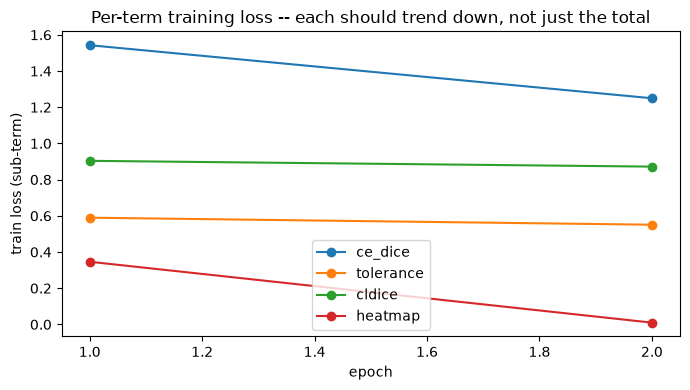
\includegraphics[width=\linewidth]{figures/joint_training_subterm_curves.png}
  \Description{Line chart of four per-term training loss curves (ce\_dice, tolerance, cldice,
  heatmap) over 2 epochs. All four lines slope downward; the heatmap curve drops most steeply,
  from about 0.35 to about 0.01.}
  \caption{Per-term training loss over 2 epochs --- all four sub-terms decrease, not just the
  total; \texttt{heatmap} drops most sharply (a $35\times$ reduction).}
  \label{fig:joint-subterms}
\end{figure}

\textbf{Verification passed}: all four sub-terms decreased epoch-over-epoch, not just the total
(Figure~\ref{fig:joint-subterms}) --- \texttt{heatmap} dropped the most sharply ($0.346 \to 0.010$,
a $35\times$ reduction), consistent with the model quickly learning that predicting near-zero
point probability almost everywhere is a strong early strategy given how sparse real point
coverage is even within Potsdam patches.

\begin{table}
  \caption{Joint model test-set evaluation, split by source, via \texttt{evaluate\_all()} with
  \texttt{point\_classes=[3]} and a 4-class \texttt{dtaf1\_config}.}
  \label{tab:joint-test}
  \begin{tabular}{@{}lcc@{}}
    \toprule
    Metric & SpaceNet-only ($n{=}19$) & Potsdam-only ($n{=}5$) \\
    \midrule
    \texttt{cbhm} & $0.144 \pm 0.115$ & $0.000 \pm 0.000$ \\
    \texttt{cbhm\_soft} & $0.230 \pm 0.119$ & $0.078 \pm 0.159$ \\
    \texttt{dtaf1} & $0.304 \pm 0.157$ & $0.092 \pm 0.149$ \\
    \texttt{dtaf1\_weighted} & $0.371 \pm 0.212$ & $0.076 \pm 0.158$ \\
    \texttt{cldice\_mean} & $0.173 \pm 0.141$ & $0.000 \pm 0.000$ \\
    \texttt{bf\_mean} & $0.252 \pm 0.151$ & $0.078 \pm 0.159$ \\
    \texttt{point\_f1\_mean} & --- & $0.200 \pm 0.447$ \\
    \bottomrule
  \end{tabular}
\end{table}

\textbf{Verification passed}: \texttt{point\_f1\_mean} is non-\texttt{None} for 5/5 real stitched
Potsdam test tiles (values $[0.0, 0.0, 0.0, 1.0, 0.0]$) --- the first time
\texttt{evaluate\_all()}'s \texttt{point\_classes} argument has ever been exercised end-to-end on
a real trained model's output, not left \texttt{None}.

\textbf{Baseline comparison}: the raw \texttt{data/train\_unet\_test\_results.csv} this session's
\texttt{train\_unet.ipynb} would produce was not present in this environment (that baseline was
originally run in an earlier session; only its already-documented aggregate survives,
Table~\ref{tab:unet-baseline}: \texttt{cbhm} $0.316\pm0.126$, \texttt{dtaf1} $0.440\pm0.134$, 15
epochs, single-source SpaceNet-only 3-class model), so no row-matched comparison was possible this
session --- only a directional one against those published aggregates. The joint run's
SpaceNet-only \texttt{cbhm} ($0.144$) and \texttt{dtaf1} ($0.304$) both come in \textbf{lower}
than the baseline's. Read this honestly rather than as evidence the new loss underperforms: this
run trained for 2 epochs against the baseline's 15, on a bigger effective task (a 4-class head
jointly absorbing gradient from four loss terms, one of them from a source, Potsdam, contributing
under 1\% of training patches) --- an apples-to-apples epoch-matched comparison has not been run.
\textbf{Framed honestly as a pipeline sanity check, not a benchmark or an ablation claim}, matching
Section~\ref{subsec:trainedmodel-setup}'s own posture toward the baseline itself.

\begin{figure}
  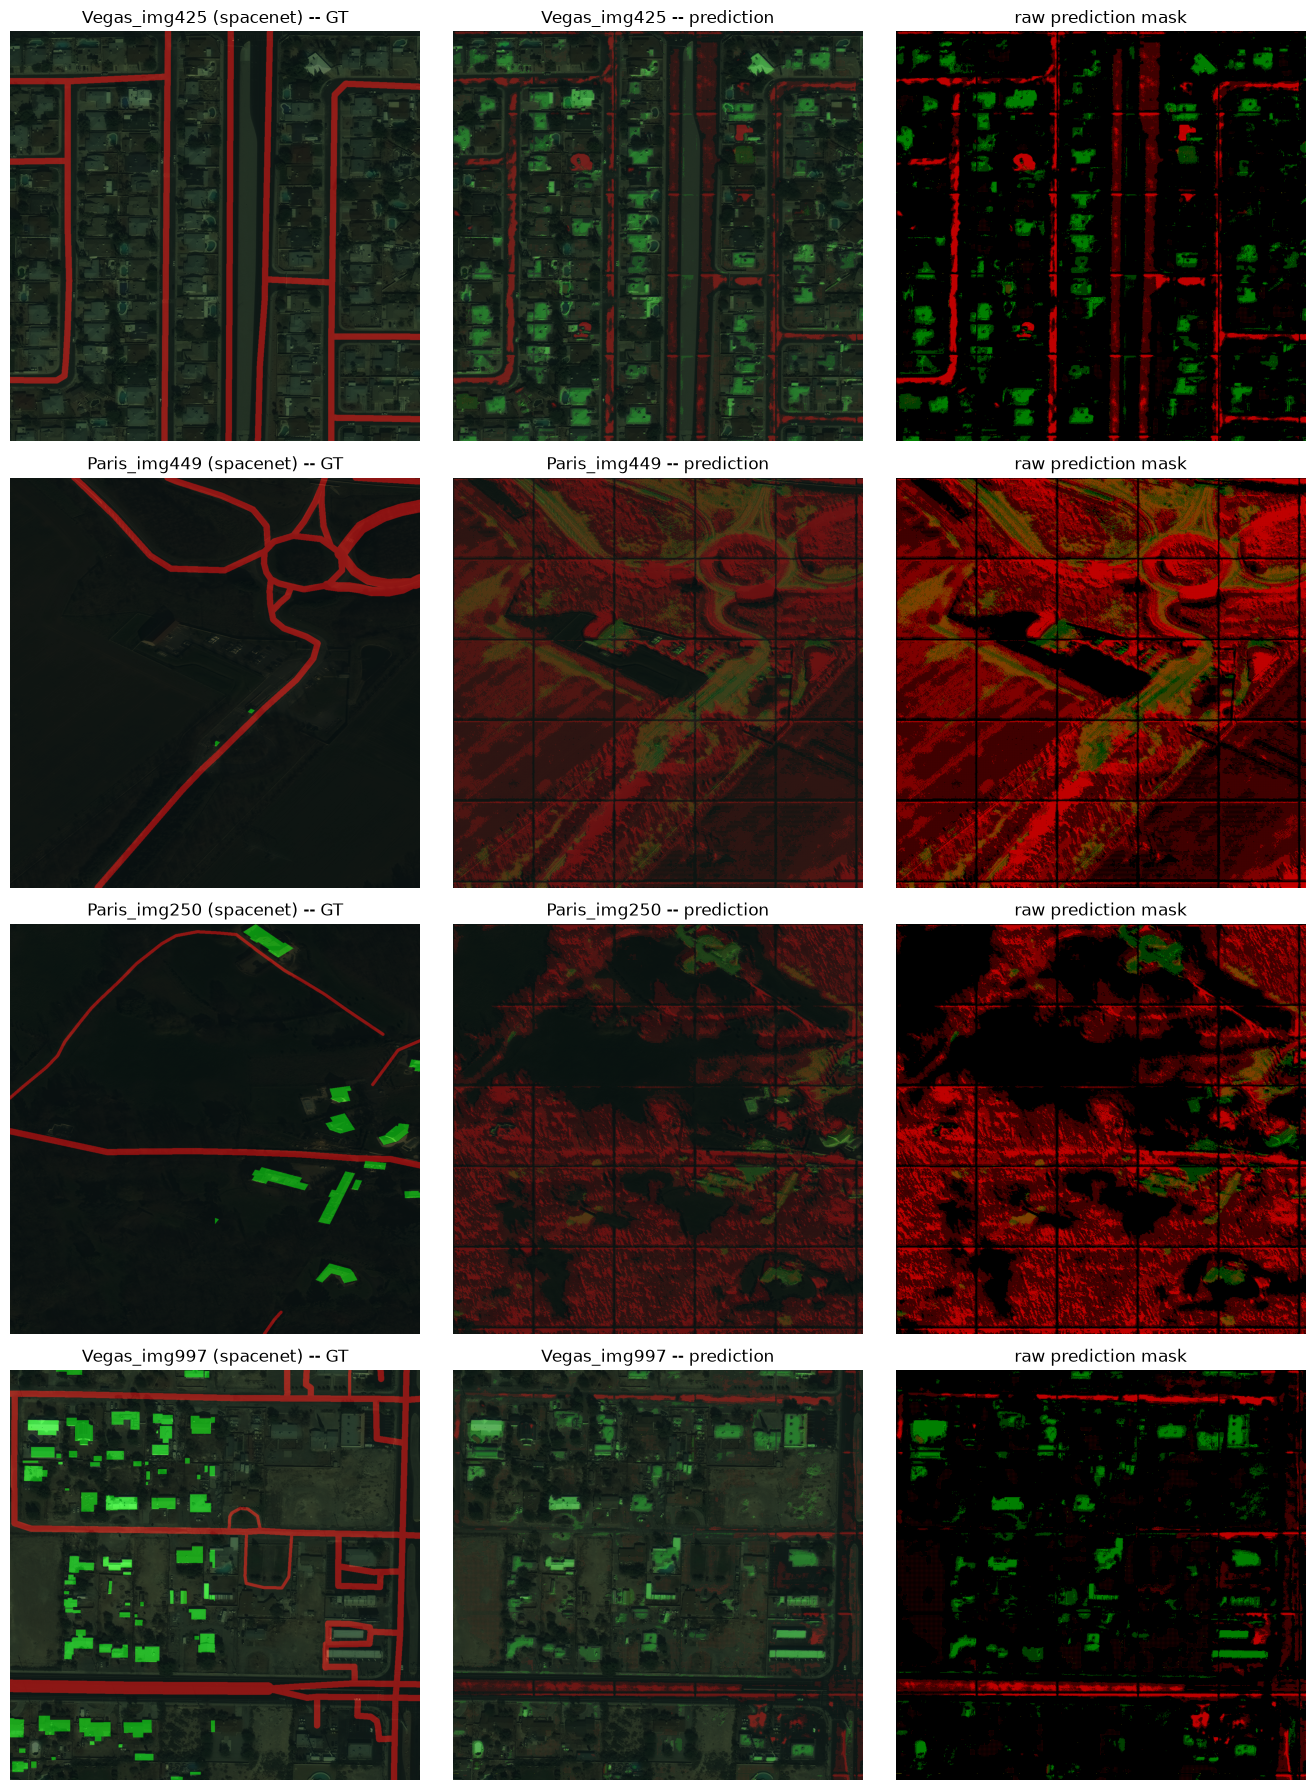
\includegraphics[width=\linewidth]{figures/joint_qualitative_panels.png}
  \Description{Four rows of three panels each (RGB image with GT overlay, RGB image with
  prediction overlay, raw prediction mask), one row per test tile, ordered worst to best by cbhm
  score: Vegas\_img425, Paris\_img449, Paris\_img250, Vegas\_img997. Roads are overlaid in red,
  buildings in green.}
  \caption{Qualitative review, worst$\to$best \texttt{cbhm} test tiles (GT / prediction / raw
  prediction mask; red$=$road, green$=$building). \texttt{Vegas\_img425} (top row, worst by
  \texttt{cbhm}) is visually one of the better-looking predictions --- see text for why its score
  is nonetheless exactly 0. \texttt{Paris\_img449}/\texttt{Paris\_img250} over-predict road across
  open terrain with no GT road, consistent with an underfit 2-epoch model.}
  \label{fig:joint-qualitative}
\end{figure}

\textbf{Qualitative review} (Figure~\ref{fig:joint-qualitative}, 4-color panels, worst$\to$best
\texttt{cbhm} tiles): mixed quality, as expected at 2 epochs, and one genuinely interesting
real-data finding. The \textbf{worst}-scoring tile by \texttt{cbhm} (\texttt{Vegas\_img425},
$\mathrm{cbhm}=0.000$) is visually one of the \emph{better}-looking predictions in the panel ---
road centerlines and building footprints are both recognizable and roughly aligned with GT. The
per-metric breakdown explains the apparent contradiction and is a real-data echo of
Section~\ref{subsec:cbhm}'s own ``harsh vs.\ lenient foil'' story: $\mathrm{bf\_mean}=0.000$
exactly (building Boundary F1, tolerance 2px, collapsed completely) while
$\mathrm{dtaf1\_weighted}=0.902$ and $\mathrm{cldice\_mean}=0.474$ are both high --- CBHM's
harmonic mean zero-collapses the \emph{entire} tile score from one class's tight-tolerance metric
hitting exactly zero, even though the lenient, tolerance-based DTAF1 view and the road-only clDice
view both say this tile is mostly correct. This is the first time that exact zero-collapse
mechanism (Appendix~\ref{app:a3}) has been observed on a real trained model's output rather than
only in synthetic scenes (Table~\ref{tab:failure-modes}) or GT-vs-perturbed-GT sweeps
(Section~\ref{subsec:realdata-results}). The best-scoring shown tile (\texttt{Vegas\_img997},
$\mathrm{cbhm}=0.364$) has a more balanced per-metric profile ($\mathrm{dtaf1}=0.402$,
$\mathrm{cldice\_mean}=0.336$, $\mathrm{bf\_mean}=0.397$) --- no single class collapsing, road and
building both partially but not perfectly recovered. The two weakest-looking predictions in the
panel (\texttt{Paris\_img449}, \texttt{Paris\_img250}) show substantial over-prediction of the
road class across open/agricultural terrain that has no GT road, consistent with an underfit
model at this epoch budget, not a structural failure of the joint loss or masking scheme. No
qualitative evidence of a masking bug (e.g.\ a SpaceNet tile hallucinating point-class
predictions, which would indicate \texttt{class\_mask} leaking) was observed in any reviewed
panel.

\section{Discussion \& Limitations}
\label{sec:discussion}

\begin{itemize}
  \item DTAF1's road-breakage blind spot (Sections~\ref{subsec:motivation-results},
    \ref{subsec:blindspot}) is fixed by DTAF1-Topo (Section~\ref{subsec:dtaf1topo}), but
    DTAF1-Topo is validated on \textbf{synthetic data only} --- not yet re-run on the real 24-tile
    sample (Section~\ref{subsec:realdata-results}'s Finding \#1), and not yet wired into
    \texttt{evaluate\_all()}.
  \item \texttt{cbhm\_soft} (Section~\ref{subsec:weighted-reduction}) only helps when the failing
    class is also the pixel-count minority; when a class sparse by \emph{area} is not sparse by
    \emph{pixel count} (\texttt{Khartoum\_img371}), the fix is partial.
  \item clDice is brittle on short/sparse real road segments --- moderate offsets can collapse it
    to exactly 0 even when DTAF1 degrades gracefully. Neither composite is uniformly more
    trustworthy --- recommend reporting \texttt{cbhm}, \texttt{cbhm\_soft}, \texttt{dtaf1}, and
    \texttt{dtaf1\_weighted} together, not picking one.
  \item U-Net results (Section~\ref{subsec:unet-results}) are a pipeline sanity check (small
    dataset, no pretraining, CPU-only), not a benchmark result --- do not oversell.
  \item APLS (Section~\ref{subsec:apls}) here is a raster-skeleton approximation, not true
    vector-graph APLS, because no vector road graph survives the \texttt{rasterize\_lines} step
    anywhere in the pipeline (Section~\ref{sec:implementation}).
  \item The harmonic-blend asymmetry proved in Section~\ref{subsec:dtaf1topo} (DTAF1-Topo can only
    ever pull a score \emph{down} toward APLS, never up) is intentional, but means DTAF1-Topo
    inherits every one of APLS's own failure modes (e.g., a genuinely correct but very
    short/sparse road segment with too few sampled control-point pairs to estimate APLS reliably)
    --- not yet characterized empirically.
  \item \textbf{\texttt{losses/} has no connectivity term, by design, not oversight.}
    APLS/DTAF1-Topo have no tractable lightweight differentiable relaxation --- graph shortest-path
    recomputation over a fragmenting skeleton graph has no obvious continuous relaxation without
    essentially reinventing a differentiable flow/graph formulation, a substantially larger
    undertaking than the other three terms. A model trained with \texttt{PLEMMultiTaskLoss}
    therefore has no direct training pressure toward connectivity, only toward tolerance-band
    coverage and centerline topology at \texttt{SoftClDiceLoss}'s fixed-iteration granularity ---
    it may still learn to produce broken roads that happen to look locally correct, exactly the
    failure mode Section~\ref{subsec:blindspot} formalizes on the eval side. Whether
    \texttt{SoftClDiceLoss} alone provides enough indirect connectivity pressure in practice is an
    open empirical question for Section~\ref{subsec:joint-results}'s real training run.
  \item \textbf{\texttt{PointHeatmapLoss} is a genuine train/eval formulation mismatch, not a
    relaxation.} Point F1 (Section~\ref{subsec:pointf1}) is evaluated via Hungarian instance
    matching at test time but trained via dense heatmap regression
    (Section~\ref{subsec:heatmap-loss}) --- these are different algorithms with different failure
    modes, so a model minimizing the heatmap loss is not directly minimizing anything Point F1
    measures, only something correlated with it. This mismatch is inherent to point supervision
    (Section~\ref{sec:method}'s assessment found no tractable differentiable relaxation of
    Hungarian matching itself), not a shortcut taken for convenience.
  \item \textbf{The tolerance-band recall direction turned out fully differentiable, not merely
    approximated.} Initial design assessment (before implementation) expected the recall direction
    would need a detached/stop-gradient hard-threshold approximation, mirroring how a real
    Euclidean distance transform of the prediction would break differentiability. Implementation
    found a cleaner alternative --- soft-dilating the model's own continuous probability map via
    differentiable max-pool --- that avoids any detach at all (Section~\ref{subsec:tolerance-loss}).
    Recorded here because it contradicts what a reader familiar with the boundary-loss literature
    (Section~\ref{subsec:related-losses}) might expect from this term specifically.
  \item \textbf{The heatmap term's loss magnitude differs from the other three by orders of
    magnitude} under point perturbations (Sections~\ref{subsec:lossablation-setup},
    \ref{subsec:lossablation-results}) --- a real, documented property of its CornerNet-style
    focal formulation (not a bounded $[0,1]$ ratio the way the tolerance/clDice terms are), not a
    bug. \texttt{PLEMMultiTaskLoss}'s per-term \texttt{weights} dict exists specifically to
    rebalance this during real training (Section~\ref{subsec:joint-setup}); the right weighting
    has not yet been empirically tuned.
  \item \textbf{SpaceNet/Potsdam are not resampled to a common GSD}
    (Section~\ref{subsec:joint-setup}) --- a Potsdam training patch covers a much smaller physical
    area than a SpaceNet patch at the same pixel size. Section~\ref{subsec:joint-results}'s run did
    not surface an obvious failure mode from this (no qualitative evidence the model confuses the
    two regimes), but a rigorous test of whether it matters would need an ablation isolating GSD
    from every other confound, not yet run.
  \item \textbf{Section~\ref{subsec:joint-results}'s real training run cannot separate ``the new
    loss underperforms'' from ``2 epochs on a harder task underperforms.''} Its SpaceNet-only
    aggregate scores ($\mathrm{cbhm}=0.144$, $\mathrm{dtaf1}=0.304$) come in below the CE+Dice
    baseline's 15-epoch numbers ($\mathrm{cbhm}=0.316$, $\mathrm{dtaf1}=0.440$,
    Section~\ref{subsec:unet-results}), but the joint run trained for 2 epochs (an explicit,
    CPU-only-time-budget scope choice) against a strictly harder task (4-class head, four combined
    loss terms, a second heterogeneous data source contributing under 1\% of training patches). No
    epoch-matched comparison exists yet --- treat the current numbers as evidence the pipeline runs
    correctly end-to-end, not as a verdict on the new loss's quality relative to CE+Dice; the
    highest-priority future-work item (Section~\ref{sec:conclusion}) is closing this gap.
  \item \textbf{A pathological-scaling guard was added to \texttt{gt\_centroids\_to\_heatmap} during
    this pipeline's integration testing}: profiling the real joint-training run surfaced that a
    synthetic worst-case target (dense, non-blob-like point-class noise, never produced by real
    Potsdam labels) could drive the per-centroid Python loop underlying the heatmap target
    construction to thousands of connected components, stalling a single training batch for
    minutes. A \texttt{max\_instances} cap (default 100 --- generous relative to real Potsdam
    crops, which top out around two dozen instances per tile) bounds this worst case with a
    one-time warning rather than a silent multi-minute stall, at the cost of dropping excess
    instances beyond the cap on malformed input. Recorded here as a concrete instance of the more
    general caution in Section~\ref{subsec:heatmap-loss}: this term's cost scales with instance
    \emph{count}, not just image size, unlike the other three terms.
\end{itemize}

\section{Conclusion \& Future Work}
\label{sec:conclusion}

This paper makes two contributions that reinforce each other. The evaluation half
(Sections~\ref{sec:evalprotocol}--\ref{sec:topological}) is a class-agnostic, tolerance/topology-aware
metric library that found and fixed two real failure modes through an explicit
synthetic-sweep $\to$ real-data validation $\to$ targeted additive fix $\to$ regression-test loop.
The training half (Section~\ref{sec:method}) asks whether the same geometric properties that
motivate those metrics can be trained \emph{into} a model directly, rather than only measured
afterward: \texttt{PLEMMultiTaskLoss} combines three differentiable analogs of those metrics
(tolerance, topology, and --- via a genuine reformulation rather than a relaxation ---
point-instance localization) into one multi-task loss, with a masked multi-source training scheme
letting datasets that individually annotate only two of three feature types jointly supervise one
4-class model. Section~\ref{subsec:lossablation-results}'s synthetic ablations confirm each term
encodes the geometric sensitivity it was designed to; Section~\ref{subsec:joint-results}'s small
real joint-training run across 153 real tiles confirms the mechanism holds together end-to-end on
real, messy imagery --- all four loss terms learn jointly, per-source masking behaves correctly,
and point-feature evaluation flows all the way through the metric library on a real trained
model's output for the first time --- the same posture Section~\ref{subsec:trainedmodel-setup}'s
original CE+Dice U-Net took toward the evaluation metrics themselves. Whether the new loss
\emph{improves on} CE+Dice, as opposed to merely working correctly, remains open pending an
epoch-matched comparison (below).

Future work:
\begin{itemize}
  \item Run an epoch-matched (or otherwise fairly controlled) comparison between the CE+Dice
    baseline and the new joint loss (highest priority ---
    Section~\ref{subsec:joint-results}'s 2-epoch run cannot separate ``the new loss is worse''
    from ``2 epochs on a harder task is worse,'' and every other item below benefits from having
    that real comparison to react to).
  \item Wire \texttt{dtaf1\_topo} into \texttt{evaluate\_all()} and \texttt{metrics/\_\_init\_\_.py}
    after real-data validation (Section~\ref{subsec:realdata-results}'s Finding \#1,
    Section~\ref{sec:discussion}).
  \item Re-run \texttt{dtaf1\_topo}/\texttt{apls} on the real 24-tile SpaceNet sample already used
    for every other real-data finding, closing the ``synthetic-only'' caveat in
    Sections~\ref{subsec:dtaf1topo}/\ref{sec:discussion}.
  \item Train on the full SpaceNet corpus with GPU/pretraining
    (Sections~\ref{subsec:trainedmodel-setup}/\ref{subsec:unet-results}), and correspondingly
    scale up the joint training run beyond a pipeline sanity check once its basic mechanics are
    confirmed.
  \item Extend the point-feature pipeline (both eval, Section~\ref{subsec:pointf1}, and training,
    Section~\ref{subsec:heatmap-loss}) to more Potsdam classes (cars).
  \item Explore learned/adaptive tolerance radii instead of fixed per-class constants
    (Section~\ref{subsec:tolerance-radii}), and correspondingly a learned rather than fixed
    \texttt{iters} for \texttt{SoftClDiceLoss} (Section~\ref{subsec:cldice-loss}).
  \item Characterize DTAF1-Topo's inherited APLS failure modes on short/sparse real road segments
    (Section~\ref{sec:discussion}'s last point) with a dedicated sensitivity sweep, mirroring
    \texttt{sweep\_sparse\_class\_offset}'s treatment of CBHM's analogous weakness
    (Section~\ref{subsec:class-imbalance}).
  \item Empirically tune \texttt{PLEMMultiTaskLoss}'s per-term \texttt{weights} dict
    (Section~\ref{sec:discussion}) once real training results are available to optimize against,
    rather than the default equal weighting used for the ablations in
    Section~\ref{subsec:lossablation-results}.
  \item Investigate whether \texttt{SoftClDiceLoss} alone provides meaningful indirect
    connectivity pressure during training (Section~\ref{sec:discussion}), as a cheaper partial
    substitute for the connectivity term \texttt{losses/} otherwise cannot have
    (Sections~\ref{subsec:apls}/\ref{subsec:method-principle}).
\end{itemize}


\begin{acks}
Parts of the implementation, notebooks, and the working outline behind this paper were developed
with the assistance of Claude Code, and were checked and are the responsibility of the author(s).
\end{acks}

\bibliography{refs}

\appendix
\section{Formal Properties and Proof Sketches}
\label{app:proofs}

One short proof per Section~\ref{sec:evalprotocol} eval-metric primitive, matching the exact
parameterizations used there. \texttt{losses/}'s terms are not given formal proofs here ---
Section~\ref{sec:method}'s claims are validated empirically, via the unit tests in
Section~\ref{sec:results}/\texttt{tests/test\_losses\_sanity.py} and the ablation sweeps in
Sections~\ref{subsec:lossablation-setup}--\ref{subsec:lossablation-results}, rather than proven;
this is noted explicitly rather than left implicit.

\subsection{Shared Edge-Case Correctness}
\label{app:a1}

\textbf{Claim:} every primitive in Section~\ref{sec:evalprotocol} returns $1.0$ when both $P_c$
and $G_c$ are empty, and $0.0$ when exactly one is empty.

\textbf{Proof sketch:} verified by direct inspection of the identical guard pattern in each
implementation --- \texttt{dtaf1.py:43-51} ($n_{\mathrm{pred}}=0$ and $n_{\mathrm{gt}}=0 \to$ all
of precision/recall/f1 $=1.0$; either alone zero $\to$ all $0.0$), \texttt{cldice.py:51-56},
\texttt{boundary\_f1.py:68-72} (same shape, on skeleton and boundary pixel counts respectively),
\texttt{point\_f1.py:109-120} (on instance counts), and \texttt{apls.py:141-144} (on foreground
pixel counts, prior to any graph construction). Since every downstream composite (CBHM,
DTAF1-Topo, \texttt{cbhm\_soft}) is built from weighted means and harmonic means of these
primitives, this shared base case is what makes ``both classes vacuously correct'' a well-defined
$1.0$ at every level of the library, not just at the leaves.

\subsection{DTAF1 Boundedness and Reduction Equivalence}
\label{app:a2}

\textbf{Claim:} $\mathrm{dtaf1\_macro}$, $\mathrm{dtaf1\_weighted} \in [0,1]$ always; and
$\mathrm{dtaf1\_weighted} = \mathrm{dtaf1\_macro}$ when GT pixel counts are equal across all
classes in \texttt{class\_config}.

\textbf{Proof sketch:} each per-class $F1_c$ is itself a harmonic mean of two quantities in
$[0,1]$ (Section~\ref{subsec:dtaf1}), hence $F1_c \in [0,1]$; both the unweighted mean
(\texttt{dtaf1.py:124}) and the pixel-count-weighted mean (\texttt{dtaf1.py:125-127}) are convex
combinations of the $F1_c$ values, hence also in $[0,1]$. When every class's $n_c$ (GT pixel
count) is equal, the weights $n_c / \sum n_c$ reduce to $1/|C|$ for every class, making the
weighted sum numerically identical to the unweighted mean.

\subsection{CBHM Zero-Collapse}
\label{app:a3}

\textbf{Claim:} $\mathrm{cbhm}=0$ if and only if $\mathrm{clDice}_{\mathrm{mean}}=0$ or
$\mathrm{BF}_{\mathrm{mean}}=0$ (or both).

\textbf{Proof sketch:} directly from \texttt{unified.py:80-81} --- $\mathrm{score} =
2 \cdot \mathrm{cl\_mean} \cdot \mathrm{bf\_mean} / \mathrm{denom}$ if $\mathrm{denom}>0$ else
$0.0$. If either $\mathrm{cl\_mean}$ or $\mathrm{bf\_mean}$ is exactly 0, the numerator is 0 while
$\mathrm{denom}$ is the other (generally nonzero) term, so $\mathrm{score}=0$ exactly ---
regardless of how close to 1 the other mean is. Conversely, if both means are strictly positive,
both numerator and denominator are strictly positive, so $\mathrm{score}>0$. This is the formal
statement behind Table~\ref{tab:failure-modes}'s ``Road shifted 5px'' row ($\mathrm{clDice}=0$
forces $\mathrm{CBHM}=0$ even though $\mathrm{DTAF1}=1.000$ on the identical input).

\subsection{\texttt{cbhm\_soft} Non-Collapse}
\label{app:a4}

\textbf{Claim:} $\mathrm{cbhm\_soft}=0$ only if \emph{both} $\mathrm{cl\_mean\_weighted}=0$ and
$\mathrm{bf\_mean\_weighted}=0$ (unlike CBHM's single-sided collapse in
Section~\ref{app:a3}).

\textbf{Proof sketch:} from \texttt{unified.py:102}, $\mathrm{cbhm\_soft} = w_{\mathrm{cl}} \cdot
\mathrm{cl\_mean\_weighted} + w_{\mathrm{bf}} \cdot \mathrm{bf\_mean\_weighted}$ is a weighted
arithmetic mean with non-negative weights summing to 1 (or 0.5/0.5 when both totals are 0). A
weighted arithmetic mean of two non-negative terms is 0 only if every term with positive weight is
itself 0. Since $w_{\mathrm{cl}}, w_{\mathrm{bf}} \ge 0$ and at least one is strictly positive
whenever any GT pixels exist, $\mathrm{cbhm\_soft}=0$ requires whichever of
$\mathrm{cl\_mean\_weighted}$/$\mathrm{bf\_mean\_weighted}$ has positive weight to be 0 --- and if
only one type is present (the other has zero GT pixels and thus zero weight),
$\mathrm{cbhm\_soft}$ simply equals that one type's weighted mean, never forced toward 0 by the
\emph{other}, absent type. This is the mechanism behind the
\texttt{Khartoum\_img371}/\texttt{Khartoum\_img333} contrast in Section~\ref{subsec:weighted-reduction}:
\texttt{cbhm\_soft} can only be dragged down by a failing class in proportion to that class's own
pixel-count weight, not collapsed outright by it.

\subsection{APLS Score Boundedness}
\label{app:a5}

\textbf{Claim:} every per-pair APLS score, and hence the aggregate \texttt{apls} score, lies in
$[0,1]$.

\textbf{Proof sketch:} each per-pair score is either $0.0$ (unmatched, \texttt{apls.py:181}) or
$\max(0.0, 1.0 - |\mathrm{pred\_len} - \mathrm{gt\_len}|/\mathrm{gt\_len})$
(\texttt{apls.py:185}) --- the outer $\max(0.0, \cdot)$ clamps the lower bound, and the term
inside is $\le 1.0$ whenever $\mathrm{pred\_len} \ge 0$ (shortest-path lengths are non-negative by
construction), so every individual score lies in $[0,1]$. The aggregate \texttt{apls} score is
\texttt{np.mean(scores)}, a convex combination of values in $[0,1]$, hence itself in $[0,1]$.

\subsection{Point F1: Hungarian Optimality vs.\ Greedy Suboptimality}
\label{app:a6}

\textbf{Claim:} there exist configurations of GT/predicted point centroids where greedy
nearest-neighbor matching strictly under-counts true positives relative to the Hungarian
assignment used in \texttt{point\_f1} (\texttt{point\_f1.py:58-65}).

\textbf{Proof sketch (formalizing \texttt{TestPointInstanceMatching}'s adversarial case):}
consider two GT points $g_1, g_2$ and one predicted point $p$ positioned such that
$\mathrm{dist}(g_1,p) < \mathrm{dist}(g_2,p)$ but a \emph{second} predicted point $p'$ exists with
$\mathrm{dist}(g_2,p') < \mathrm{tolerance}$ while $\mathrm{dist}(g_1,p') > \mathrm{tolerance}$. A
greedy matcher processing predictions in an order that assigns $p \to g_1$ first (the globally
nearer pair) can leave $g_2$ unmatched to $p'$ if it was already ``claimed'' --- or, in the
canonical clustered-points case, greedy assigns the single nearest GT to \emph{both} predictions'
shared nearest neighbor, yielding $\mathrm{TP}=1$. The Hungarian assignment instead minimizes
total assignment cost over the \emph{complete} bipartite graph simultaneously
(\texttt{linear\_sum\_assignment} on the full cost matrix), correctly recovering the one-to-one
pairing $p{\leftrightarrow}g_1, p'{\leftrightarrow}g_2$ that gives $\mathrm{TP}=2$ --- strictly
more true positives from the same input, because it considers all pairings jointly rather than
greedily committing to the locally-best match first. This is also the formal reason
Section~\ref{subsec:heatmap-loss} does not attempt a differentiable relaxation of Hungarian
matching for the training loss: the property that makes it correct (global joint optimization
over the complete bipartite graph) is exactly the discrete, combinatorial structure that has no
useful gradient.

\section{Algorithms and Computational Complexity}
\label{app:complexity}

One subsection per Section~\ref{sec:evalprotocol} primitive gives its per-primitive computational
complexity. Sections~\ref{app:b8}--\ref{app:b12} extend this to the four \texttt{losses/} terms
from Section~\ref{sec:method}, on the same basis: cost per forward pass on one batch of $H\times W$
tiles, in the same $N$/$k$ notation as Section~\ref{app:b1}.

\subsection{General Framework and Notation}
\label{app:b1}

Let $N=H\times W$ be the pixel count of one tile, and (where relevant) $k$ the number of
point-class instances in a scene (typically tens to low hundreds, $k \ll N$). For
Sections~\ref{app:b8}--\ref{app:b12}, $B$ is batch size and $\mathrm{iters}$ is a loss term's
fixed iteration count.

\subsection{DTAF1}
\label{app:b2}
Two calls to \texttt{scipy.ndimage.distance\_transform\_edt}, each $O(N)$ (the exact Euclidean
distance transform algorithm used by SciPy runs in linear time via a two-pass separable
algorithm); TP/precision/recall computation is a constant number of $O(N)$ boolean-mask
reductions. Total per class: $O(N)$.

\subsection{clDice}
\label{app:b3}
\texttt{skimage.morphology.skeletonize} (Lee's thinning algorithm) is near-linear in $N$; the
subsequent set intersections are $O(N)$. Total per class: $O(N)$.

\subsection{Boundary F1}
\label{app:b4}
Morphological boundary extraction (\texttt{binary\_dilation} with a small structuring element) is
$O(N)$; two \texttt{distance\_transform\_edt} calls are $O(N)$ each as in Section~\ref{app:b2}.
Total per class: $O(N)$.

\subsection{Point F1}
\label{app:b5}
Connected-component labeling (\texttt{scipy.ndimage.label}) is $O(N)$. The subsequent Hungarian
assignment (\texttt{linear\_sum\_assignment}) operates on a $k\times k$ cost matrix and runs in
$O(k^3)$ --- cheap in practice since $k$ is an \emph{instance} count, not a pixel count, making
this the one primitive in the library whose dominant cost term is independent of $N$ for
realistic point-class densities.

\subsection{APLS}
\label{app:b6}
Skeletonization is $O(N)$ as in Section~\ref{app:b3}; building the 8-connected adjacency graph is
a single pass over skeleton pixels, $O(N)$. Control-point pairs are sampled grouped by source
specifically so that \texttt{nx.single\_source\_dijkstra\_path\_length} --- run once per unique
sampled source at $O((V+E)\log V)$ where $V,E$ are the skeleton graph's node/edge counts --- is
amortized across many targets per source rather than paying one independent Dijkstra call each per
sampled \emph{pair}. With $n_{\mathrm{pairs}}$ total pairs grouped into $O(\sqrt{n_{\mathrm{pairs}}})$
sources (the default sampling policy), this reduces total Dijkstra work from
$O(n_{\mathrm{pairs}} \cdot (V+E)\log V)$ (naive) to $O(\sqrt{n_{\mathrm{pairs}}} \cdot (V+E)\log V)$.
cKDTree snap-matching is $O(\log V)$ per query after an $O(V\log V)$ tree build.

\subsection{DTAF1-Topo / \texttt{cbhm\_soft}}
\label{app:b7}
Both composites add no new asymptotic cost beyond summing their already-analyzed constituent
primitives' costs: DTAF1-Topo is \texttt{dtaf1()} ($O(N)$ per class, Section~\ref{app:b2}) plus
\texttt{apls\_multiclass()} (Section~\ref{app:b6}) plus an $O(|\mathrm{linear\_classes}|)$
harmonic-mean blending pass --- no additional raster-level work. \texttt{cbhm\_soft} is a handful
of extra $O(1)$-per-class weighted-sum arithmetic operations on scores CBHM already computes ---
strictly cheaper than either primitive it reweights.

\subsection{\texttt{ToleranceBandLoss}}
\label{app:b8}
The GT-side dilation-by-radius is $O(\mathrm{radius} \cdot B N)$: $\mathrm{radius}$ sequential
$3\times3$ max-pool passes, each $O(BN)$. The recall direction's soft-dilation of the prediction is
the identical operation applied to a continuous tensor instead of a binary one, same
$O(\mathrm{radius} \cdot BN)$ cost. Precision/recall ratio computation is $O(BN)$ per class. Total
per class: $O(\mathrm{radius} \cdot BN)$ --- in the same $O(N)$-per-tile family as DTAF1
(Section~\ref{app:b2}), with $\mathrm{radius}$ (typically 2--10, Section~\ref{subsec:tolerance-radii})
as a small constant multiplier, and cheaper per-call in practice than DTAF1's exact Euclidean
distance transform (Section~\ref{app:b2}'s two-pass separable algorithm has a larger constant
factor than repeated $3\times3$ max-pooling for the tolerance radii actually used in this paper).

\subsection{\texttt{SoftBoundaryLoss}}
\label{app:b9}
The morphological-gradient boundary map is two $3\times3$ pooling passes, $O(BN)$. The remainder
of the computation is exactly \texttt{ToleranceBandLoss}'s primitive (Section~\ref{app:b8})
applied to this boundary map instead of the full class mask, so total per class:
$O(\mathrm{radius} \cdot BN)$, identical complexity family to Section~\ref{app:b8} with a small
constant-factor overhead for the boundary-map computation itself.

\subsection{\texttt{SoftClDiceLoss}}
\label{app:b10}
Each soft-erode/soft-dilate/soft-open call is one $3\times3$ pooling pass, $O(BN)$; soft
skeletonization performs $\mathrm{iters}$ such passes (default $\mathrm{iters}=10$), so
skeletonization is $O(\mathrm{iters} \cdot BN)$. This runs once for the prediction and once for GT
(the GT skeletonization is computed under \texttt{no\_grad}, but has the same forward-pass cost).
The $\mathrm{tprec}$/$\mathrm{tsens}$ ratio computation is $O(BN)$ per class. Total per class:
$O(\mathrm{iters} \cdot BN)$ --- same asymptotic family as Section~\ref{app:b3}'s near-linear
\texttt{skimage.skeletonize}, with $\mathrm{iters}$ playing the role of Section~\ref{app:b3}'s
(implicit, converge-to-completion) iteration count, except fixed rather than input-dependent ---
the direct computational reason for Section~\ref{subsec:cldice-loss}'s iteration-bounded
width-invariance limitation.

\subsection{\texttt{PointHeatmapLoss}}
\label{app:b11}
Target construction (\texttt{gt\_centroids\_to\_heatmap}) is $O(N)$ per sample for the
Gaussian-burn step plus \texttt{scipy.ndimage.label} + \texttt{center\_of\_mass}'s $O(N)$
connected-component pass (identical cost profile to Section~\ref{app:b5}'s centroid extraction,
here used for target construction rather than eval-time matching) --- no $O(k^3)$ Hungarian term,
since this loss performs no assignment at all (Section~\ref{subsec:heatmap-loss}). More precisely,
the per-centroid Gaussian-burn loop is $O(k' \cdot N)$ where $k'$ is the (capped, see
Section~\ref{sec:discussion}) number of connected components in that sample --- realistic
point-feature data keeps $k' \ll N$, but this is the one \texttt{losses/} term whose cost scales
with instance \emph{count} rather than purely with image size, unlike
Sections~\ref{app:b8}--\ref{app:b10}. \texttt{heatmap\_focal\_loss} itself is $O(BN)$, a constant
number of pointwise tensor operations.

\subsection{\texttt{PLEMMultiTaskLoss}}
\label{app:b12}
No new asymptotic cost beyond summing Sections~\ref{app:b8}--\ref{app:b11}'s already-analyzed
constituent costs plus the base CE+Dice term ($O(BN)$, standard cross-entropy and soft-Dice
computation) --- the pre-softmax class-masking step is a single $O(BC)$-broadcast addition,
negligible next to any of the per-pixel terms. Total: $O(\mathrm{iters} \cdot BN + k' N)$,
typically dominated by \texttt{SoftClDiceLoss}'s iteration-bounded skeletonization
(Section~\ref{app:b10}) unless a sample's point-instance count $k'$ is unusually large.


\end{document}
